%\documentclass[xcolor=dvipsnames,9pt]{beamer} 
\documentclass[xcolor=dvipsnames,9pt,hide notes,mathserif]{beamer}
%\documentclass[xcolor=dvipsnames,9pt,handout,hide notes,mathserif]{beamer}

\usepackage{pgfpages}
\usepackage{listings}
%\usepackage{enumitem}
\newtheorem{Fact}[theorem]{Fact}

%% For creating a handout:
\mode<handout>{\pgfpagesuselayout{4 on 1}[border shrink=5mm]
  \pgfpageslogicalpageoptions{1}{border code=\pgfusepath{stroke}}
  \pgfpageslogicalpageoptions{2}{border code=\pgfusepath{stroke}}
  \pgfpageslogicalpageoptions{3}{border code=\pgfusepath{stroke}}
  \pgfpageslogicalpageoptions{4}{border code=\pgfusepath{stroke}}
}

%% For creating notes for the speaker:
%\setbeameroption{notes on second screen}
%\setbeameroption{show notes}

\setbeamerfont{structure}{family=\rmfamily,shape=\scshape} 
\usepackage{graphicx}
\usepackage{tikz}
\usepackage{scalefnt}
\usepackage{amsmath}%
\usepackage{amsfonts}%
\usepackage{amssymb}%
%(wjd) added stmaryrd and enumerate packages
\usepackage{stmaryrd,enumerate}
\usepackage{graphicx}
\usepackage{comment}
\usetikzlibrary{matrix,arrows}
\usepackage{ulem}
\usepackage{mathrsfs,textcomp}
\setbeamertemplate{navigation symbols}{}
\usepackage{verbatim}
\usepackage{xspace}
\usepackage[mathcal]{euscript}
\usepackage[smaller]{acronym}
\acrodef{lics}[LICS]{Logic in Computer Science}

%% \usepackage{euler} 
\usepackage[T1]{fontenc}
\usepackage[english]{babel}
\usepackage[latin1]{inputenc}
\usepackage{times}
% Or whatever. Note that the encoding and the font should match. If T1
% does not look nice, try deleting the line with the fontenc.

% This changes the color of alerted text to blue:
\definecolor{MyDarkBlue}{rgb}{0.2,0.2,0.7}
\definecolor{olivegreen}{cmyk}{0.64,0,0.95,0.40} % PANTONE 582
\setbeamercolor{alerted text}{fg=blue}
\newcommand{\emphcyan}[1]{\textcolor{MyDarkBlue}{\textbf{#1}}}
%\renewcommand{\alert}[1]{\textcolor{olivegreen}{\emph{#1}}}
%% \renewcommand{\alert}[1]{\textcolor{olivegreen}{{\it #1}}}
\renewcommand{\alert}[1]{\textcolor{olivegreen}{#1}}
%\renewcommand{\alert}[1]{\textbf{{\emph{#1}}}}
% (default is red, but my slides are green and I don't like red and green together)

%\usecolortheme[named=OliveGreen]{structure} 
\usecolortheme[named=olivegreen]{structure} 
\setbeamertemplate{items}[square] 
\setbeamertemplate{blocks}[rounded][shadow=false]
\renewcommand{\emph}[1]{\alert{{\it #1}}}

\usepackage{inputs/wjd}

\mode<presentation>{\usetheme{boxes}}  %boxes,Pittsburgh JuanLesPins, PaloAlto, Singapore, Szeged, Warsaw, Boadilla
%\usetheme{Madrid}}
%\usetheme{boxes}  %boxes,Pittsburgh JuanLesPins, PaloAlto, Singapore, Szeged, Warsaw, Boadilla


\title{The Rectangularity Theorem \\
  {\large of Libor Barto and Marcin Kozik}\\
  {\small with applications to small CIBs}}
\author[William DeMeo]{William DeMeo\\
  {\small \url{williamdemeo@gmail.com}}\\[4pt]
  %  {\small Iowa State University}\\[4pt]
  {\footnotesize joint work with}\\[4pt] 
  Cliff Bergman and Josh Thompson
}
\institute{Iowa State University}

\date[Boulder 2016]{ % (optional, should be abbreviation of conference name)
  Workshop on Algebras and Algorithms\\{\small University of Colorado, Boulder, May 19--22}\\[6pt]
}

\subject{Universal Algebra; Lattice Theory; CSP.}% (optional) inserted into PDF info catalog.

\begin{document}
\thicklines

%% \includeonlyframes{titlepage,intro,intro2,intro3,intro4,intro5,intro6,problem1,cib,general1,cube,cp,general2,remaining,examples1,examples2,examples3,examples4,others}
%%\includeonlyframes{intro6}


\frame[label=titlepage]{
  \titlepage
  \hfill {\footnotesize slides available at\\ 
    \hfill \url{https://github.com/williamdemeo/Talks}}
}


%%%%%%%%%%%%%%%%%%%%%%%%%%%%%%%%%%%%%%%%%%%%%%%%%%%%%%%%%%%
%% 1: CSP Intro 1
\frame[label=intro]{
  \frametitle{Definition of CSP}
  \framesubtitle{(naive version)}
  
  {\bf Input}
  \begin{itemize}
  \item \emph{variables:} $\sV = \{v_1, v_2, \dots\}$
  \item \emph{domain:}  $\sD$
  \item \emph{constraints:} $C_1, C_2, \dots$
  \end{itemize}
  \vskip1cm
  %  \underline{Output}
      {\bf Output}
      \begin{itemize}
      \item ``yes'' if there is a \emph{solution}  
        \[
        f : \sV \rightarrow \sD \quad 
        \text{    {\small (an assignment of values to variables that satisfies all $C_i$)}}
        \] 

      \item ``no'' otherwise
      \end{itemize}

}


\begin{frame}
  \frametitle{Definition of CSP}
  \framesubtitle{(jaded version)}

  $\bA = \<A, \sF\>$ is a finite idempotent algebra,
  $\Sub(\bA)$ is all subuniverses of $\bA$. \\[4pt]

  {\it In this talk} $\CSP(\bA)$ denotes the following decision problem:

  \bigskip
  
  An \defn{instance of degree} $n$ of $\CSP(\bA)$ is the tuple $\<\sV, \sA, \sS, \sR\>$ 
  \begin{itemize}
  \item \emph{variables} $\sV = \{0, 1, \dots, n-1\}$;\\[4pt]
  \item \emph{domains} $\sA = \{\bA_0, \bA_1, \dots, \bA_{n-1}\} \subset \Sub(\bA)$  (one for each variable)\\[4pt]
  \item \emph{scope functions} $\sS = (\bs_0, \bs_1, \dots, \bs_{p-1})$ 
    with \emph{constraint arities} $\ar(\sS) = (m_0, m_1, \dots, m_{p-1})$;\\[4pt]
  \item \emph{constraint relations} $\sR = (\bR_0, \bR_1, \dots, \bR_{p-1})$, where
    \[\bR_i \leq \bA_{\bs_i(0)} \times \bA_{\bs_i(1)}\times \cdots \times \bA_{\bs_i(m_i-1)}.\]
  \end{itemize}
  
  \bigskip
  
  A \defn{solution} to $\<\sV, \sA, \sS, \sR\>$ is an assignment
  $f: \sV \to A$ of values to variables that satisfies all constraints. That is,
  \[f\in \myprod_{\sV}A_j
  \quad  \text{and} \quad 
  \Proj_{\bs_i} f \in \bR_i, \;\text{ for each $0\leq i < p$.}\]

  \onslide<2>{ {\bf Notation:} $\nn = \{0,1,\dots, n-1\}$, so the $i$-th scope
    has type $\bs_i : \mm_i \to \nn$ and
    \[ \Proj_{\bs_i} f  = f \circ \bs_i \]}
\end{frame}

\begin{frame}
  \frametitle{Example 1}
  \framesubtitle{...thanks, Ross!}

  Let $\bA=\<\{0,1\}, \{f\}\>$, where
  \[f(x,y,z) = x+y+z \pmod 2.\]

  Consider the ternary relations
  \[  R_0 = \{(0,0,0), (1,1,0), (1,0,1), (0,1,1) \}\]
  \[ R_1 =  \{(1,0,0), (0,1,0), (0,0,1), (1,1,1) \}\]
  %% \begin{align*}
  %%   R_0 &= \{(x,y,z)\in \{0,1\}^3: f(x,y,z)=0 \}\\
  %%   &= \{(0,0,0), (1,1,0), (1,0,1), (0,1,1) \}
  %% \end{align*}
  %% \begin{align*}
  %%   R_1 &= \{(x,y,z)\in \{0,1\}^3: f(x,y,z)=1\}\\
  %%   & = \{(1,0,0), (0,1,0), (0,0,1), (1,1,1) \}
  %% \end{align*}

  \onslide<2->{Each $\bR_i=\<R_i, \{f\}\>$ is a subalgebra of $\bA^3$}
  \onslide<3->{...in fact, they're subdirect.}

  \smallskip

  \onslide<3->{\hfill {\bf notation:} $\bR_i \sdp \bA^3$\phantom{XXXXXXX}}

  \bigskip

  \onslide<4->{So we have a degree 3 instance of $\CSP(\bA)$, where
    \begin{itemize}
    \item \alert{variables:} $\sV = \{0,1,2\}$
    \item \alert{domains:} $A_i =\{0,1\}, \quad i = 0,1,2$
    \item \alert{scope functions:} the identity on $\{0,1,2\}$
    \item \alert{constraint relations:} $\bR_0$ and $\bR_1$
    \end{itemize}
  }
\end{frame}

\tikzstyle{lat} = [circle,draw,inner sep=0.8pt]
\begin{frame}
  \frametitle{Example 1}
  \framesubtitle{$\cap$ and potatoes}
  \begin{center}
    \begin{tikzpicture}[scale=1]
          \draw (0,.5) ellipse (4mm and 12mm);
    \draw (2,.5) ellipse (4mm and 12mm);
    \draw (4,.5) ellipse (4mm and 12mm);
    \node[lat] (00) at (0,0) {};
    \node[lat] (01) at (0,1) {};
    \node[lat] (10) at (2,0) {};
    \node[lat] (11) at (2,1) {};
    \node[lat] (20) at (4,0) {};
    \node[lat] (21) at (4,1) {};
    \draw (00) node [below]{$0$};
    \draw (01) node [above]{$1$};
    \draw (10) node [below]{$0$};
    \draw (11) node [above]{$1$};
    \draw (20) node [below]{$0$};
    \draw (21) node [above]{$1$};

      \draw[red,thick] (00) -- (10) -- (20);
      \draw[blue,thick] (00) -- (11) -- (21);
      \draw[green,thick] (01) -- (10) -- (21);
      \draw[yellow,thick] (01) -- (11) -- (20);
      \draw (6.5,0.5) node {(lines are elements of $R_0$)};
    \end{tikzpicture}
    %% \nopagebreak[4]
    \vskip2mm
    \begin{tikzpicture}[scale=1]
          \draw (0,.5) ellipse (4mm and 12mm);
    \draw (2,.5) ellipse (4mm and 12mm);
    \draw (4,.5) ellipse (4mm and 12mm);
    \node[lat] (00) at (0,0) {};
    \node[lat] (01) at (0,1) {};
    \node[lat] (10) at (2,0) {};
    \node[lat] (11) at (2,1) {};
    \node[lat] (20) at (4,0) {};
    \node[lat] (21) at (4,1) {};
    \draw (00) node [below]{$0$};
    \draw (01) node [above]{$1$};
    \draw (10) node [below]{$0$};
    \draw (11) node [above]{$1$};
    \draw (20) node [below]{$0$};
    \draw (21) node [above]{$1$};

      \draw[yellow,thick] (01) -- (11) -- (21);
      \draw[red,thick] (00) -- (10) -- (21);
      \draw[green,thick] (01) -- (10) -- (20);
      \draw[blue,thick] (00) -- (11) -- (20);
      \draw (6.5,0.5) node {(lines are elements of $R_1$)};
    \end{tikzpicture}
  \end{center}
  \medskip
  \onslide<2->{Notice for all $i, j \in \{0,1,2\}$,
    \[\Proj_{ij}R_0 = \Proj_{ij}R_1\]}
  \onslide<3->{\hfill    ...yet $R_0 \cap R_1 = \emptyset$. \phantom{XXXXXXX} }

\end{frame}

\begin{frame}
  \frametitle{Example 2}
  \framesubtitle{...thanks, Cliff!}
  
  Let $\bA = \<\{0,1\}, \{m\}\>$, where $m: A^3 \to A$ is a majority operation, 
  \[m(x,x,y)\approx m(x,y,x)\approx m(y,x,x) \approx x.\]
  
  Let $\bR_0, \bR_1 \sdp \bA^3$ with universes
  \begin{align*}
    R_0 &= \{(0,0,0), (0,0,1), (0,1,0), (1,0,0)\},\\
    R_1 &= \{(0,1,1), (1,0,1), (1,1,0), (1,1,1)\}.
  \end{align*}

  This describes the instance of $CSP(\bA)$ with
  \begin{itemize}
  \item \alert{variables:} $\sV = \{0,1,2\}$
  \item \alert{domains:} $A_i =\{0,1\}, \quad i = 0,1,2$
  \item \alert{scope functions:} the identity on $\{0,1,2\}$
  \item \alert{constraint relations:} $\bR_0$ and $\bR_1$
  \end{itemize}
\end{frame}
\begin{frame}
  \frametitle{Some conveniences}

  Retrict attention to instances where all constraint relation are
  subdirect,
  
  \[\bR_i \sdp \bA_{\bs_i(0)} \times \bA_{\bs_i(1)}\times \cdots \times \bA_{\bs_i(m_i-1)}\]

  \bigskip
  \onslide<2->{Could visualize $(\bs_i, \bR_i)$ as specifying a subalgebra
    of the full product $\myprod_{\sV}\bA_j$ 
    \[\lb \bs_i, \bR_i\rb = \{\ba \in \myprod_{j\in \sV}A_j \mid \Proj_{\bs_i}\ba \in \bR_i\}\]
\hfill {\small (thanks again, Ross!)} \phantom{XX}

\medskip

Convenient because now solutions are the elements in
    $\bigcap_{i\in V}\lb \bs_i, \bR_i\rb$.}

  \bigskip

  \onslide<3->{
    BUT input size is not a function of these ``full'' subdirect products!
  }

  \medskip

  \onslide<3->{(Input size could be defined as the length of a string of
    all tuples in scopes and constraint relations of the instance.)}
\end{frame}

\begin{frame}
  \frametitle{End of Act I}
  \framesubtitle{first intermission}
  pause...

  \bigskip

  \onslide<1->{\hfill ...draw more potatoes... \phantom{XXXXXXXXXXXXXXXXXXXXXXXXX}}

  \bigskip

  \onslide<1->{ \hfill ...give audience chance to escape.}
\end{frame}

\begin{frame} \frametitle{Absorption Theory {\small (for mortals)}}
%  \framesubtitle{Definitions}
  Let $\bA = \<A, F^{\bA}\>$ be a finite algebra in a Taylor variety.

  \bigskip

  Let $t\in \Clo(\bA)$ be a $k$-ary term operation.

  \bigskip

  A subalgebra  %% $\bB = \<B, F^{\bB}\> \leq \bA$ is
  $\bB \leq \bA$ is 
  {\it \alert{absorbing} in $\bA$ with respect to $t$} if 
  \[a\in A, \; b_i \in B \quad \Longrightarrow  \quad
  t^{\bA}(b_0, \dots, b_{j-1}, a, b_{j+1}, \dots, b_{k-1})\in B  \quad (\text{all } j\in \kk)
  \]
  \onslide<2->{%
    Equivalently, $t^{\bA}[B^{j-1}\times A \times B^{k-j}] \subseteq B$,  for all
    $0\leq j < k$, that is,
    \[(\bb, \ba, \bb')\in B^{j-1}\times A \times B^{k-j} \quad \Longrightarrow  \quad
    t^{\bA}(\bb, \ba, \bb')\in B.
    \]}
  \onslide<3->{%
    {\bf Notation:}

    \medskip
    $\bB \absorbing \bA$ means $\bB$ is absorbing in $\bA$ with respect to some term.

    \medskip

    To be explicit about the term, $\bB \absorbing_t \bA$.

    \bigskip

    %% Call $t$ an ``absorbing term'' for $\bB$ in this case.
    %% \bigskip
 
    $\bB \minabsorbing \bA$ means $\bB\absorbing \bA$ and
    $B$ is minimal (with respect to inclusion)
    among absorbing subuniverses of $\bA$. 

    \bigskip
    
    An algebra is \defn{absorption-free} (AF) if it has no proper absorbing
    subalgebras.
  }
\end{frame}

\begin{frame}
  \frametitle{Where are we going with this?}
  
  ``The Absorption Theorem'' of Barto and Kozik (LMCS 2012)

  \bigskip

  Concerns the special class of ``linked'' subdirect products.  

  \bigskip

  {\it Identifies some special cases in which a subdirect product is the full product!}

  \onslide<2->{
  \begin{theorem}[Absorption Theorem]
    If $V$ is an idempotent locally finite variety, then TFAE
    \begin{itemize}
    \item $V$ is a Taylor variety;
    \item if $\bA_0, \bA_1 \in V$ are finite idempotent absorption-free algebras 
      and $\bR \sdp \bA_0 \times \bA_1$ is linked, then $\bR = \bA_0 \times \bA_1$.
    \end{itemize}
  \end{theorem}
  }
  \onslide<3->{
    At Vanderbilt Shanks Workshop (2015),
    Barto presented more joint work with Kozik 
    generalizing the Absorption Theorem to more than two factors.

    \bigskip

    The ``Rectangularity Theorem'' 
    says roughly$^\ast$, a subdirect product of simple nonabelian algebras 
    contains the full product of minimal absorbing subalgebras.
  }

  \onslide<4->{
   \hfill {\small $^\ast$assuming suitable conditions under which the theorem is true.}
    }

  
\end{frame}
  

\begin{frame}
  \frametitle{Linked subdirect products}
  A subdirect product $\bR \sdp \bA_0 \times \bA_1$ is \alert{linked} if
  for all $a, a' \in \Proj_0 R$,
  
  \[\exists\; c_0, c_2, \dots, c_{2n} \in A_0, \quad
  \exists\; c_1, c_3, \dots, c_{2n+1} \in A_1\]
  such that
  \[
  a = c_0, \quad
  (c_{2i},c_{2i+1})\in R,\quad
  (c_{2i+2},c_{2i+1})\in R,\quad c_{2n} = a'
  \]

  %% \begin{align*}
  %% c_0 &= a, \\
  %% (c_{2i},c_{2i+1})&\in R,\\
  %% (c_{2i+2},c_{2i+1})&\in R,\\
  %% c_{2n} &= a'
  %% \end{align*}

  \bigskip
  \onslide<2->{
  %% \hfill  ...potatoes anyone? \phantom{XXXXXXXXXXXXXX}

  
\includegraphics[height=3cm]{inputs/amconfus.png}

  \hfill  {\small [todo: insert potato diagram]} \phantom{XXXXXXXXXXXXXX}
  }
\end{frame}


\begin{frame}
  \frametitle{Linked subdirect products}
  \framesubtitle{for algebraists}
  {\bf Notation:}

  \medskip
  For $\bR \sdp \bA_0 \times \bA_1$, let $\etaR_i$ denote the kernel of the
  $i$-th projection of $\bR$. That is,
  \[
  \etaR_i = \ker(\bR \onto \bA_i) = \{(\br, \br')\in R^2 \mid \Proj_i \br =
  \Proj_i \br'\}
  \]
  Let $R^{-1} = \{(y,x) \in A_1 \times A_0 \mid (x,y) \in R\}$.

  \bigskip
  \onslide<2->{
  The following are equivalent:
  \begin{itemize}
  \item $\bR \sdp \bA_0 \times \bA_1$ is linked;
  \item $\etaR_0\join \etaR_1 = 1_R$;
  \item if $a, a' \in \Proj_0 R$, then $(a,a')$ is in the transitive closure of $R\circ R^{-1}$.
  \end{itemize}
  }

  \bigskip


\end{frame}
%%%% ALTERNATIVE (SHORTER) VERSION:
%% It is easy to see that if
%% $\bR \sdp \bA_0 \times \bA_1$ and $\etaR_i := \ker(\bR \onto \bA_i)$, then 
%% $\bR$ is linked if and only if
%% $\etaR_0\join \etaR_1 = 1_R$.
\begin{frame} \frametitle{Properties of Absorption I}
Absorption has nice properties...
  \begin{itemize}
  \item (transitivity) $\bC \absorbing \bB \absorbing \bA \; \Longrightarrow \; \bC \absorbing \bA$
  \item (closure under nonempty $\cap$ and finite products)
    
    \medskip
    If $\bB \absorbing_f \bA$ and $\bC \absorbing_g \bA$ and $B \cap C\neq \emptyset$, then 
    $\bB \cap \bC\absorbing \bA$.
    %$ is absorbing in $

    \medskip

    If $\bB_0 \absorbing_f \bA_0$ and $\bB_1 \absorbing_g \bA_1$,
    then $\bB_0\times \bB_1 \absorbing_t \bA_0\times \bA_1$. 
    %% $\bB_0\times \bB_1$ is absorbing in $\bA_0\times \bA_1$ with respect to $f\star g$.

    \smallskip
    {\small ...with respect to $t = f\star g$ in both cases.}

    \medskip
    
  \end{itemize}

  \begin{overprint}
    \onslide<2|handout:1>
    
        If $f: A^\ell\to A$ and $g: A^m\to A$, then
        $f \star g$  is the $\ell m$-ary operation 
        \[f(g(a_{1 1}, \dots, a_{1 m}), g(a_{2 1}, \dots, a_{2 m}), \dots,  g(a_{\ell 1}, \dots, a_{\ell m}))\]
    \onslide<3-|handout:2>
    More generally, 
    if $\bB_i\absorbing_{t_i}\bA_i$ for $0\leq i < n$, then
    $\myprod \bB_i \absorbing_s \myprod \bA_i$.
    
    %% If $\bB_i\absorbing_{t_i}\bA_i$ (resp, $\bB_i\minabsorbing_{t_i}\bA_i$) for each $0\leq i < n$,
    %% then

    %% \medskip
    %% $\myprod \bB_i \absorbing_s \myprod \bA_i$ (resp, $\myprod \bB_i \minabsorbing_s \myprod \bA_i$) 
    \smallskip
    {\small ...with respect to $s= t_0\star t_1 \star \cdots \star t_{n-1}$.}

    \bigskip
    An obvious but important consequence:
    \begin{center}
    {\it A finite product of finite idempotent algebras is AF if each factor is AF.}
    \end{center}
  \end{overprint}
  \onslide<4|handout:2>{
    \bigskip
        {\bf Restriction Lemma.}
        
      If $\bB \absorbing_t \bA$ and $\bC \leq \bA$ and $D = B\cap C \neq \emptyset$,
      then $\bD\absorbing \bC$ with respect to the restriction of $t$ to $C$.
  }
\end{frame}

\begin{frame} \frametitle{Properties of Absorption II}
  \framesubtitle{LSD Lemmas}
    
\begin{lemma}[LSD 1]
\label{lem:gen-abs1}
If $\bB_i\absorbing \bA_i$ and $\bR \leq \myprod_{i}\bA_i$ and $R':= R \cap \myprod_i B_i \neq \emptyset$,
then %$\bR \cap \myprod_i \bB_i\absorbing \bR$.
$\bR'\absorbing \bR$.
\end{lemma}
{\it Proof.}  $\myprod \bB_i \absorbing_t \myprod \bA_i$, 
{\small  so follows Restriction Lemma if we put} $C = R$.

  \begin{lemma}[LSD 2]
    \label{lem:sdp-general}
    Suppose $\bB_i \minabsorbing \bA_i$ and  $\bR \sdp \myprod \bA_i$.
    If $R' := R \cap \myprod B_i \neq \emptyset$, then  
    $\bR' \sdp \myprod \bB_i$.
  \end{lemma}

  \begin{lemma}[LSD 2]
    \label{lem:linked-absorber}
    If $\bR \sdp \bA_0 \times \bA_1$ is linked and 
    $\bS \absorbing \bR$, then $\bS$ is linked.
  \end{lemma}

  
\end{frame}
\begin{frame} \frametitle{Linking is easy}
  \framesubtitle{...sometimes}
  %% When can we expect a subdirect product to be \emph{linked}, as is required 
  %% of $\bR \sdp \bA_0\times \bA_1$ in the statement of the Absorption Theorem?
  In some simple cases we get linking from LSD Lemmas along with 
  the following elementary

  \bigskip
  
  {\bf Fact.}  Suppose $\bR \sdp \bA_0 \times \bA_1$ and let $\etaR_i = \ker(\bR \onto \bA_i)$.
    \begin{enumerate}
    \item 
      If $\bA_0$ is simple, then either $\etaR_0 \join \etaR_1 = 1_R$ or $\etaR_0 \geq \etaR_1$.
    \item If $\bA_0$ and $\bA_1$ are both simple, then either $\etaR_0 \join \etaR_1 = 1_R$
      or $\etaR_0 = 0_R = \etaR_1$.
    \end{enumerate}
  
  \bigskip
  ...so, if both factors are simple, then $\etaR_0 \neq \etaR_1$ gives the linking...

  \bigskip
{\bf Cor 1.}    Let $\bA_0$ and $\bA_1$ be simple. If  $\bR \sdp \bA_0\times \bA_1$
and $\etaR_0 \neq \etaR_1$, then $\bR$ is linked.

  \bigskip

...and if one factor is simple nonabelian and the other abelian, linking is free! 

  \bigskip
{\bf Cor 2.}  If $\bA_0$ is simple nonabelian and $\bA_1$ abelian, then
    every subdirect product of $\bA_0 \times \bA_1$ is linked.

    %% \onslide<2->{
    %%   Moreover, if 
    %%   $\bR \sdp \bA_0 \times \bA_1$ and if $\bB_0 \minabsorbing \bA_0$,
    %%  then  $\bR$ intersects $\bA_0\times \bB_1$ nontrivially and this intersection
    %% forms a linked subdirect product of $\bA_0 \times \bB_1$.}

\end{frame}

%% \begin{frame}  \frametitle{Properties of Absorption III}\end{frame}

\begin{frame} \frametitle{Absorption Theorem: Application}
  Suppose we add to the respective contexts of the last three results the hypothesis
  that the algebras live in an idempotent variety with a Taylor term...

  \bigskip  
  (We will refer to such varieties as ``Taylor varieties'' and we call the
  algebras they contain ``Taylor algebras.'')

  \bigskip  
  ...then the Absorption Theorem (in combination with facts above) yields

  \bigskip  
  {\bf Lemma:}
  Let $\bA_0$ and $\bA_1$ be finite Taylor algebras
  with $\bB_i\minabsorbing \bA_i$ ($i =0,1$)
  and suppose $\bR \sdp \bA_0 \times \bA_1$ and $\etaR_0 \neq \etaR_1$.
    \begin{enumerate}[(i)]
    \item If $\bA_0$ and $\bA_1$ are simple and $R\cap (B_0 \times B_1) \neq \emptyset$, then
      $\bB_0 \times \bB_1\leq \bR$. 
    \item  If $\bA_0$ is simple nonabelian and $\bA_1$ is abelian,
      then $\bB_0 \times \bA_1 \leq \bR$.
    \end{enumerate}

    \bigskip
    \onslide<2->{How is this relevant to CSP?}

    \bigskip
    \onslide<3->{Abelian potatoes can all go in the same sack...}

    \bigskip
    \onslide<4->{...simple nonabelian potatoes cannot.}
    
\end{frame}


\begin{frame} \frametitle{The Rectangularity Theorem}
  \framesubtitle{A Generalization of the Absorption Theorem}

  Barto and Kozik generalized the Absorption Theorem
  to multiple simple nonabelian factors. This is...
  \bigskip
  \onslide<2->{
    
  {\bf The Rectangularity Theorem.}

  \medskip
  Let $\bA_0, \bA_1, \dots, \bA_{n-1}$ be finite algebras in a 
  Taylor variety, $\bB_i \minabsorbing \bA_i$, and suppose
  \begin{itemize}
  \item at most one $\bA_i$ is abelian,
  \item all nonabelian factors are simple, 
  \item $\bR \sdp \bA_0 \times \bA_1 \times \cdots \times \bA_{n-1}$,
  \item $\etaR_i \neq \etaR_j$ for all $i\neq j$. %where $\etaR_i = \ker(\bR %\onto \bA_i)$,
  \item $\bR'= \bR \cap (\bB_0 \times \bB_1 \times \cdots \times \bB_{n-1})$ is nonempty.
  \end{itemize}
  
  \[\text{Then } \; \bR' = \bB_0 \times \bB_1 \times \cdots \times \bB_{n-1}.\] % \leq \bR$.
  }
\end{frame}


\begin{frame} \frametitle{Rectangularity Theorem}
  \framesubtitle{Proof Sketch}

  {\bf Notation:}

  \bigskip

  Let $\nn =\{0, 1, 2, \dots, n-1\}$.

  \bigskip

  Let $\sigma' = \nn -\sigma$, when $\sigma$ is a subset of $\nn$.

  \bigskip

  For $\bR \sdp \myprod_{\nn}\bA_i$ %\bA_0 \times \bA_1 \times \cdots \times \bA_{n-1}$, let 
  let
  \[
  \etaR_\sigma = \ker(R \onto \Pi_\sigma A_i) = \{(\br, \br') \in R^2 \mid
  \Proj_\sigma \br = \Proj_\sigma \br' \},
  \]


  If $\sigma\subseteq \nn$, then by
  $\bR \sdp \myprod_\sigma \bA_i \times \myprod_{\sigma'}\bA_i$ we 
  mean
  \[
  \bR\leq \myprod_{\nn} \bA_i, \quad 
\Proj_\sigma\bR = \myprod_\sigma \bA_i, \quad \text{ and }\quad
\Proj_{\sigma'}\bR = \myprod_{\sigma'} \bA_i.
\]
  and we say that $\bR$ is a \defn{subdirect product of} 
  $\myprod_\sigma \bA_i$ and $\myprod_{\sigma'}\bA_i$ in this case.

  \bigskip 

  The subdirect product $\bR \sdp \myprod_\sigma \bA_i \times
  \myprod_{\sigma'}\bA_i$ 
  is said to be \defn{linked} if $\etaR_\sigma \join \etaR_{\sigma'} = 1_R$.

  \bigskip

  We may use $\bR_\sigma$ for $\Proj_\sigma\bR$, the projection 
  of $\bR$ onto coordinates in $\sigma$.

  
\end{frame}

\begin{frame} \frametitle{Rectangularity Theorem}
  \framesubtitle{Proof Sketch}
  From now on,
    \emph{all algebras are finite and belong to the same Taylor variety}.

    \onslide<2->{    {\bf Lemma 1.}
      
    Let $\bB_i\minabsorbing \bA_i$ for each $i\in \nn $, 
    and let $\nn  = \sigma \cup {\sigma'}$ be a disjoint union.
    
    Assume $\bR$ is a \emph{linked} subdirect product of 
    $\myprod_{\sigma} \bA_i$ and $\myprod_{\sigma'}\bA_i$.
    
    Suppose $R' = R \cap \myprod_i B_i \neq \emptyset$.    Then $\bR' = \myprod_i \bB_i$.
    }

    \bigskip

    \onslide<3->{
    {\bf Lemma 2.} [Kearnes-Kiss, Thm~3.27]
    
    Suppose $\alpha$ and $\beta$ are congruences of a Taylor algebra. Then
    %% $\sansC(\alpha, \alpha; \alpha \meet \beta)$ if and only if
    %% $\sansC(\alpha \join \beta, \alpha \join \beta; \beta)$.
    \[\sansC(\alpha, \alpha; \alpha \meet \beta) \quad \Longleftrightarrow \quad
    \sansC(\alpha \join \beta, \alpha \join \beta; \beta).\]
    }
    \onslide<4->{
    %% \medskip
    %% The Kearnes and Kiss theorem can be used to prove
    %% \medskip

    {\bf Lemma 3.} [Linking Lemma]
    
    Let $n\geq 2$ %% let $\bA_0, \bA_1, \dots, \bA_{n-1}$ be finite algebras in a
    %% Taylor variety, and let 
    and $\bB_i \minabsorbing \bA_i$ for all $i\in \nn$. Suppose
    \begin{itemize}
    \item at most one $\bA_i$ is abelian
    \item all nonabelian factors are simple
    \item $\bR \sdp \bA_0 \times \bA_1 \times \cdots \times \bA_{n-1}$,
    \item $\etaR_i \neq \etaR_j$ for all $i\neq j$.
    \end{itemize}
    Then there exists $k$ such that $\bR\sdp \bA_k \times \bR_{k'}$ is linked.
}
  %% \begin{proof}
%% We have $\bR' \sdp \myprod_\sigma \bB_i \times \myprod_{\sigma'} \bB_i$, and
%% $\bR' \absorbing \bR$, so LSD 3 implies $\bR'$ is linked. 
%% Both $\myprod_{\sigma} \bB_i$ and $\myprod_{\sigma'} \bB_i$ are AF, so the Absorption
%% Theorem implies $\bR' = \myprod_{\sigma}\bB_i \times \myprod_{\sigma'}\bB_i$.
%% \end{proof}

\end{frame}

\begin{frame} \frametitle{Rectangularity Theorem}
  \framesubtitle{Proof Sketch}

    
  {\bf The Rectangularity Theorem.}

  \medskip
  Let $\bA_0, \bA_1, \dots, \bA_{n-1}$ be finite algebras in a 
  Taylor variety, $\bB_i \minabsorbing \bA_i$, and suppose
  \begin{itemize}
  \item at most one $\bA_i$ is abelian,
  \item all nonabelian factors are simple, 
  \item $\bR \sdp \bA_0 \times \bA_1 \times \cdots \times \bA_{n-1}$,
  \item $\etaR_i \neq \etaR_j$ for all $i\neq j$. %where $\etaR_i = \ker(\bR %\onto \bA_i)$,
  \item $\bR'= \bR \cap (\bB_0 \times \bB_1 \times \cdots \times \bB_{n-1})$ is nonempty.
  \end{itemize}
  
  \[\text{Then } \; \bR' = \bB_0 \times \bB_1 \times \cdots \times \bB_{n-1}.\] % \leq \bR$.

  {\bf Proof.} Induct on the number of factors in the product
  $\bA_0 \times \bA_1 \times \cdots \times \bA_{n-1}$.

  \bigskip
  For $n=2$ the result holds by earlier Lemma (slide 16).

  \bigskip

\end{frame}
\begin{frame} \frametitle{Rectangularity Theorem}
  \framesubtitle{Obstacles to Applications}

  \begin{enumerate}
  \item<1-> {\bf Nonabelian factors must be simple.}
    This is the most obvious limitation of the theorem and in general
    we don't yet have a way to overcoming it.  However, we have ideas...

  \item<2-> {\bf Abelian factors must have easy partial solutions.}
    Cor~\ref{cor:RT-cor} and \ref{cor:RT-cor-gen} assume that
    when the given constraint relations are projected onto the abelian factors,
    we already know a partial solution---that is, an element that satisfies all
    constraint relations after projecting these relations onto the abelian
    factors of the full product. 

  \item<3-> {\bf Intersecting mass products.}
    RT and corollaries assume that the universe $R$ of the subdirect
    product in question intersects nontrivially
    with a product $\myprod B_i$ of minimal absorbing subuniverses.
  \end{enumerate}

\end{frame}


\end{document}


  Fix $n>2$ and assume that for all $2 \leq k < n$ 
  the result holds for subdirect products of 
  $k$ factors. We will prove the result holds for subdirect products of 
  $n$ factors.

  Let $\sigma$ be a nonempty proper subset of $\nn$ %:=\{0, 1, \dots, n-1\}$ 
  (so $1\leq |\sigma| < n$) and let
  $\sigma'$ denote the complement of $\sigma$ in $\nn$.
  Denote by $\bR_\sigma$ the projection of $\bR$ onto the $\sigma$-factors. 
  That is, $\bR_\sigma := \Proj_\sigma \bR$ and  $\bR_{\sigma'}:=\Proj_{\sigma'} \bR$.
  Each of these projections satisfies the assumptions
  of the theorem,
  since $\bR_{\sigma} \sdp \myprod_{\sigma}\bA_i$ and since
  for all $i\neq j$ in $\sigma$, we have
  %\etaR_i \neq \etaR_j\; \iff \; 
  $\ker(R_{\sigma} \onto A_i) \neq \ker(R_{\sigma}\onto A_j)$.
  Similarly for $\bR_{\sigma'}$.
  %% \begin{equation}
  %%   \label{eq:4}
  %% %\etaR_i \neq \etaR_j\; \iff \; 
  %% \ker(R_{\sigma} \onto A_i) \neq \ker(R_{\sigma}\onto A_j).
  %% \end{equation}
  %% Similarly for $\bR_{\sigma'}$.
  %% (Let's make sure Equation (\ref{eq:4}) is as obvious as it seems:
  %% since $\etaR_i\neq \etaR_j$, either there is a pair 
  %% $(\br, \br')\in R^2\cap \etaR_i$ 
  %% that does not belong to $\etaR_j$,
  %% or there is a pair 
  %% $(\br, \br')\in R^2\cap \etaR_j$ 
  %% that does not belong to $\etaR_i$.  Without loss of generality, 
  %% assume the former, so that $r_i=r_i'$ and $r_j\neq r_j'$.  
  %% Since $i, j \in \sigma$, the projection
  %% of $\br$ and $\br'$ onto $\sigma$ will also satisfy
  %% $r_i=r_i'$ and $r_j\neq r_j'$.)
  %%
  %% Since $\bR_\sigma$ and  $\bR_{\sigma'}$ satisfy the assumptions of the theorem,
  Therefore, the induction hypothesis implies that %% \bB_{\sigma} :=
  $\myprod_{\sigma}\bB_i \leq \bR_{\sigma}$ and
  %% $\bB_{\sigma'} :=
  $\myprod_{\sigma'}\bB_i \leq \bR_{\sigma'}$.
  By Corollary~\ref{cor:min-abs-prod},
  $\myprod_{\sigma}\bB_i  \minabsorbing \myprod_{\sigma} \bA_i$, and
  since $\myprod_{\sigma}\bB_i \leq \bR_{\sigma}\leq \myprod_{\sigma} \bA_i$ 
  it's clear that  $\myprod_{\sigma}\bB_i \absorbing \bR_{\sigma}$.
  In fact, $\myprod_{\sigma}\bB_i \minabsorbing \bR_{\sigma}$ as well, 
  %% To see this,
  %%   suppose $\bS\leq \myprod_{\sigma}\bB_i$ and $\bS\absorbing \bR_{\sigma}$. Then
  %%   $\bS\absorbing \myprod_{\sigma}\bB_i$, so $\bS\absorbing \myprod_{\sigma}\bA_i$, by
  %%   transitivity of absorption. Thus, by minimality of
  %%   $\myprod_{\sigma}\bB_i \minabsorbing \myprod_{\sigma}\bA_{i}$,
  %%   we have $\bS = \myprod_{\sigma}\bB_i$, as desired.
  by minimality of
  $\myprod_{\sigma}\bB_i \minabsorbing \myprod_{\sigma}\bA_{i}$,
  and transitivity of absorption.
  To summarize, for every $\emptyset \subsetneq \sigma\subsetneq \nn$,
  \begin{equation}
    \label{eq:20}
  \bR \sdp \bR_{\sigma} \times \bR_{\sigma'}, \quad
  \myprod_\sigma \bB_i \minabsorbing \bR_{\sigma}, \quad
  \myprod_{\sigma'} \bB_i \minabsorbing \bR_{\sigma'}.
  %% \bB_{\nn } \minabsorbing \bR_{\nn } \quad \text{ and } \quad
  %% \bB_n \minabsorbing \bA_n.
  %% \bB_{\nn } \minabsorbing \bR_{\nn } \quad \text{ and } \quad
  %% \bB_n \minabsorbing \bA_n.
  \end{equation}

  Finally, by the Linking Lemma (Lem.~\ref{lem:Link-2}) there
  is a $k$ such that 
  $\bR \sdp \bR_{k} \times \bR_{k'}$ is linked.  Therefore,
  by Lemma~\ref{lem:general-linked} the
  the proof is complete.
\end{proof}

\begin{frame} \frametitle{Proof of Rectangularity Theorem I}


\end{frame}



Here is an easily proved fact that provides some equivalent ways to define ``linked.''
%% \todo{write out the proofs that these are equivalent and maybe insert them here
%%   (unless they are too simple and tedious).}

\end{frame}


  %% \bigskip
  %% You will grow tired of hearing me say,
  %% \begin{center}
  %% ``product of minimal absorbing subuniverses''
  %% \end{center}
  %% Can we agree that a {\bf M}inimal {\bf A}bsorbing {\bf S}ubuniverse is a ``\mas''?
  %% \bigskip
  %% ...and the product of \masses is a ``\mas product''?
  %% \bigskip


  
\end{frame}





\end{document}


**** Key Ingredients of Proof
***** Absorption Theorem
***** Kearnes-Kiss
**** "New" Corollaries
**** Potential Limitations (and how to overcome them)
**** Application to CIBs
** 19:54 major rewrite of algebraic-csp.tex

In \lics'10 (\cite{MR2953899}), Libor Barto and Marcin Kozik proved a powerful ``Absorption Theorem'' 

%%% example f(x,y,z) = x+y+z mod 2 (More details)

All of the facts observed above about $\bR$ are also true of $\bS$.  In
particular, $\Proj_{\{i,j\}} S = A_i \times A_j$ for 
each pair $i\neq j$ in $\{1,2,3\}$.
If both $\bR$ and $\bS$ belong to the set of relations 
(or ``constraints'') of a single $\CSP(\bA)$ instance, then the instance
has no solution since $R \cap S = \emptyset$, despite the fact that  
$\Proj_{\{i,j\}}\bR = \Proj_{\{i,j\}}\bS$  for each pair $i\neq j$ in
$\{1,2,3\}$. To put it another way, $\bR$ and $\bS$  
witness a failure of the \emph{2-intersection property}. The ``potato
diagram'' of $\bA^3$ below depicts the elements of
$R$ and $S$ as colored lines (with colors chosen to emphasize equality of
the projections onto $\{1,2\}$). 


This algebra is clearly simple and has two proper
subuniverses, $\{0\}$ and $\{1\}$, neither of which is absorbing, so $\bA$ is
absorption-free.   It's convenient to give short names to the elements of $R$.  
Let us use the integers that they (as binary tuples) represent.
That is, $0 = (0,0,0)$, $3 = (1,1,0)$,  $5 = (1,0,1)$,  and 
$6 = (0,1,1)$,   
so $R = \{0, 3, 5, 6\}$.
Let $\etaR_i = \ker(\bR \onto \bA_i)$, and identify each
congruence with the associated partition of the set $R$. Then,
%% \[\etaR_1 = |0,6|3,5|, \quad \etaR_2 = |0,5|3,6|, \quad  \etaR_3 = |0,3|5,6|, \]
$\etaR_1 = |0,6|3,5|; \,  \etaR_2 = |0,5|3,6|; \,  \etaR_3 = |0,3|5,6|$,
so $\etaR_i \meet \etaR_j = 0_R$ and $\etaR_i \join \etaR_j = 1_R$.
In fact, the three projection kernels are the only nontrivial congruence
relations of $\bR$.

\tikzstyle{lat} = [circle,draw,inner sep=0.8pt]
\begin{center}
  \begin{tikzpicture}[scale=1.2]
    \node[lat] (bot) at (0,0) {};
    \node[lat] (top) at (0,2) {};
    \node[lat] (a) at (-1,1) {};
    \node[lat] (b) at (0,1) {};
    \node[lat] (c) at (1,1) {};
    \draw[semithick] (bot) -- (a) -- (top) -- (b) -- (bot) -- (c) -- (top);
    \draw (top) node [right]{$1_R$};
    \draw (bot) node [right]{$0_R$};
    \draw (a) node [left]{$\etaR_1$};
    \draw (b) node [right]{$\etaR_2$};
    \draw (c) node [right]{$\etaR_3$};
    \draw (-2.5,1) node {$\Con(\bR) = $};
  \end{tikzpicture}
\end{center}

Each projection of $\bR$ onto 2 coordinates of $\bA^3$ is ``linked;'' 
these binary projections are all readily seen to be
$\{(0,0), (0,1), (1,0), (1,1)\} =  A \times A$ in this case. 
Lemma~\ref{lem:abs2} tells us that this must be so.  For the set 
$\{S \subseteq \nn  \mid \bigwedge_{i\in S} \etaR_i = 0_R\}$ that appears in the
lemma is, in this example,
$\sS = \{\{1,2\}, \{1,3\}, \{2,3\}, \{1,2,3\}\}$, and the projection of
$R$ onto the coordinates in each minimal  set in $\sS$ must
equal $A \times A$ by the lemma. 


















\begin{frame}
  \frametitle{Example}

  Let $\bA = \<\{0,1\}, \{m\}\>$, where $m: A^3 \to A$ is a majority operation, 
  \[m(x,x,y)\approx m(x,y,x)\approx m(y,x,x) \approx x.\]
  
  Let $\bR_0$ and $\bR_1$ be subalgebras of $\bA^3$ with universes
  \begin{align*}
    R_0 &= \{(0,0,0), (0,0,1), (0,1,0), (1,0,0)\},\\
    R_1 &= \{(0,1,1), (1,0,1), (1,1,0), (1,1,1)\}.
  \end{align*}

  This describes the instance with
  \begin{itemize}
  \item variables: $\sV = \{0,1,2\}$
  \item domains: $A_i =\{0,1\}$
  \item scope functions: both the identity on $\{0,1,2\}$
  \item constraint relations: $\bR_0$ and $\bR_1$
  \end{itemize}
\end{example}
\end{frame}




    \draw (0,.5) ellipse (4mm and 12mm);
    \draw (2,.5) ellipse (4mm and 12mm);
    \draw (4,.5) ellipse (4mm and 12mm);
    \node[lat] (00) at (0,0) {};
    \node[lat] (01) at (0,1) {};
    \node[lat] (10) at (2,0) {};
    \node[lat] (11) at (2,1) {};
    \node[lat] (20) at (4,0) {};
    \node[lat] (21) at (4,1) {};
    \draw (00) node [below]{$0$};
    \draw (01) node [above]{$1$};
    \draw (10) node [below]{$0$};
    \draw (11) node [above]{$1$};
    \draw (20) node [below]{$0$};
    \draw (21) node [above]{$1$};


  \frametitle{Example}
  \framesubtitle{...this is Cliff's (not Ross's)}
  \begin{example}
  Let $\bA = \<\{0,1\}, \{m\}\>$, where $m: A^3 \to A$ is a majority operation, that is,
  $m(x,x,y)\approx m(x,y,x)\approx m(y,x,x) \approx x$.
  Notice that
  $\{0\} \minabsorbing \bA$ and
  $\{1\} \minabsorbing \bA$.
  Let $B_0 = \{0\}$ and $B_1 = \{0\}$.  Then, for each triple $(i,j,k) \in \{0,1\}^3$,
  Corollary~\ref{cor:min-abs-prod} implies $\bB_i \times \bB_j \times \bB_k \minabsorbing \bA^3$.
  Let
  \begin{align*}
  R &= \{(0,0,0), (0,0,1), (0,1,0), (1,0,0)\},\\
  S &= \{(0,1,1), (1,0,1), (1,1,0), (1,1,1)\}.
  \end{align*}
  Then $\bR = \<R, \{m\}\>$ and $\bS=\<S, \{m\}\>$ are 
  subdirect products of $\bA^3$. %Obviously they are disjoint, $R \cap S = \emptyset$.
  Each product $B_i \times B_j \times B_k$ of minimal absorbing subuniverses of $\bA$
  intersects either $R$ or $S$, but since $R \cap S = \emptyset$, none of these
  products intersects nontrivially with both $R$ and $S$.  In such examples,
  although the Rectangularity Theorem correctly predicts that 
  $R \cap (B_i \times B_j \times B_k)\neq \emptyset$ implies
  $B_i \times B_j \times B_k \subseteq R$, we cannot use this fact to produce a
  solution to an instance of $\CSP(\bA)$ with constraint relations $\{R, S\}$.
  To draw such a conclusion, there must be a single \mas product $\myprod \bB_i$
  intersecting nontrivially with all constraint relations.

\end{example}



\note{
  In computer science, the Boolean Satisfiability Problem 
  (abbreviated as SAT) is the problem of determining if there exists an
  \emph{interpretation} that satisfies a given Boolean formula. 

  In other words, it asks whether the \emph{variables} of a given Boolean
  formula can be consistently replaced by the values TRUE or FALSE in such a
  way that the formula evaluates to TRUE. 

  If this is the case, then the formula is called \emph{satisfiable}. 
  On the other hand, if no such assignment exists, the function expressed by
  the formula is identically FALSE for all possible variable assignments and
  the formula is unsatisfiable. For example, the formula ``$x \meet \neg y$'' is
  satisfiable because one can find the values, namely $x = 1$ and $y = 0$, 
  which make $(x \meet \neg y) = 1$. 

  In contrast, ``$x \meet \neg x$'' is unsatisfiable. 
}


%%%%%%%%%%%%%%%%%%%%%%%%%%%%%%%%%%%%%%%%%%%%%%%%%%%%%%%%%%%
%% 2: CSP intro 2
\frame[label=intro2]{
  \frametitle{Constraint Satisfaction Problems}
  \framesubtitle{Example: 3-SAT}
%  \underline{Input}
  {\bf Input}
  \begin{itemize}
  \item \emph{variables:} $V = \{v_1, \dots, v_n\}$
  \item \emph{domain:} $D = \{0, 1\}$
  \item \emph{constraints:} a formula, say,
    \[
    f(v_1, \dots, v_n) = (v_1 \join v_2 \join \neg v_3) \meet 
    (\neg v_1 \join v_3 \join v_4) \meet  \cdots
    \] 
  \end{itemize}
%  \underline{Output}
 {\bf Output}
  \begin{itemize}
  \item ``yes'' if there is a solution:  $\sigma : V \rightarrow D$ such that
    \[
    f(\sigma v_1,\dots, \sigma v_n) = 1
    \]
  \item ``no'' otherwise
  \end{itemize}
}

%%%%%%%%%%%%%%%%%%%%%%%%%%%%%%%%%%%%%%%%%%%%%%%%%%%%%%%%%%%
%% 3: CSP intro 3
\frame[label=intro3]{
  \frametitle{Constraint Satisfaction Problems}
  \framesubtitle{Example: NAE-SAT}
%  \underline{Input}
  {\bf Input}
  \begin{itemize}
  \item  \emph{variables:} $V = \{v_1, \dots, v_n\}$
  \item \emph{domain:} $D = \{0, 1\}$
  \item \emph{constraints:} $(s_1,C_1), (s_2,C_2),\dots $ {\small of the form}
    \begin{align*}
    s &= (i, j, k) \in \{1, \dots, n\}^3  \qquad \text{ {\small (scopes)}}\\
    C &= \neg (v_i = v_j = v_k)%  \qquad \text{ {\small (constraints)}}
    \end{align*}
    %% $(s_1,C_1), (s_2,C_2), \dots$ where 
    %% \begin{itemize}
    %% \item $s_i = (i_1, i_2, i_3) \in [n]^3$ {\small ``scopes''}
    %% \item $C_i = \neg (v_{i_1} = v_{i_2} = v_{i_3})$
    %% \end{itemize}
  \end{itemize}
  \onslide<2->
  In terms of relational structures...
  \begin{align*}
  \text{Let } \quad S &:= \{(v_i, v_j, v_k) : (i, j, k) 
  \text{ {\small is a scope} }\}
  \subseteq V^3\\
  R &:= \{(0,0,1), (0,1,0), (0,1,1), (1,0,0), (1,0,1), (1,1,0)\}
  \subseteq D^3
  \end{align*}
  %% \end{overprint}
\onslide<3->
  Then a solution $\sigma$ must satisfy
  ``$\sigma S \subseteq R$''
\[
\text{that is, } \quad (x,y,z) \in S \; \Longrightarrow \;
(\sigma x, \sigma y, \sigma z) \in R
\]
\onslide<4->
\emph{Solutions are homomorphisms!}
\[\sigma : \<V, S\> \rightarrow \<D, R\>\]
}

%%%%%%%%%%%%%%%%%%%%%%%%%%%%%%%%%%%%%%%%%%%%%%%%%%%%%%%%%%%
%% 4: CSP intro 4
\frame[label=intro4]{
  \frametitle{CSP: relational formulation}

  Let $\bbD = \<D, \sR\>$ be a relational structure.\\[4pt]
  $\CSP (\bbD)$ (or $\CSP(\sR)$) is the decision problem with\\[6pt]
%  \underline{Input}
  {\bf Input}
  \begin{itemize}
  \item  A structure $\bbV = \<V, \sC\>$ \emph{similar}  to $\bbD$.
  \end{itemize}
%  \underline{Output}
 {\bf Output}
  \begin{itemize}
  \item ``yes'' if there is a homomorphism $\sigma : \bbV \rightarrow \bbD$
  \item ``no'' otherwise
  \end{itemize}
\vskip5mm

  \begin{overprint}
  \onslide<2|handout:1>
  Alternatively, let $\Rightarrow$ be the binary relation on
  similar structures:
  \[
  \bbV \Rightarrow \bbD \quad 
  \text{ iff there is a homomorphism $\sigma: \bbV \rightarrow \bbD$}
  \]
  Then the CSP of $\bbD$ is the membership problem for the set
  \[
  \CSP(\bbD) := \{\bbV : \bbV \Rightarrow \bbD\}
  \]
  \onslide<3|handout:2>
  We call $\bbD$ (or $\sR$) ``tractable'' if there is a
  polynomial-time algorithm for solving
  $\CSP(\bbD)$ (or $\CSP(\sR)$).
  %%  in time polynomial in the size of $\bbV$.
  %% any instance $\bbV$\\ 
  %%   of $\CSP(\bbD)$ in time polynomial in the size of $\bbV$.
  \end{overprint}
}

%%%%%%%%%%%%%%%%%%%%%%%%%%%%%%%%%%%%%%%%%%%%%%%%%%%%%%%%%%%
%% 5: CSP intro 5
\frame[label=intro5]{
%  \frametitle{Constraint Satisfaction Problems}
  \frametitle{CSP: algebraic formulation}

  Let $\bbD = \<D, \sR\>$ be a relational structure. \\[4pt]
  For $R \subseteq \sR$ %of relations on $D$, 
  define the \emph{polymorphisms} of $R$,
  \[
  \sansPoly(R) := \{f:D^k \rightarrow D \mid
  f(\rho)\subseteq \rho \text{ {\small for every} } \rho \in R \}
  \]
  \begin{overprint}
  \onslide<2|handout:1>
  that is, 
    $f\in \sansPoly(R)$ iff for every $\rho\in R$ %{\small (say, $n$-ary)}
  \vskip2mm 
  \begin{tabular}{rcl}
    $(a_1, b_1, \dots, z_1)$ &$\in$ & $\rho$\\
    &$\vdots$ & \\
    $(a_k, b_k, \dots, z_k)$ & $\in$ & $ \rho$\\[1mm]
    \hline\\[-2mm]
    $(f(a_1, \dots, a_k), \dots, f(z_1, \dots, z_k))$ & $\in $ & $\rho$
  \end{tabular}
  \onslide<3|handout:2>
  \vskip4mm
  Define the algebra $\bD := \<D, \sansPoly(R)\>$.\\[6pt]  
  We call $\bD$ ``tractable'' if the corresponding 
  structure $\<D, R\>$ is tractable.
  \end{overprint}

}

%%%%%%%%%%%%%%%%%%%%%%%%%%%%%%%%%%%%%%%%%%%%%%%%%%%%%%%%%%%
%% 6: CSP intro 6
\frame[label=intro6]{
%  \frametitle{Constraint Satisfaction Problems}
  \frametitle{CSP: algebraic formulation}

  \onslide<1-> For $F$ a set of operations on $D$,
  define the \emph{relational clone} of $F$,
  \[
  \sansRel(F) := \{\rho \subseteq D^n \mid
  f(\rho)\subseteq \rho \text{ for every } f \in F \}
  \]
  Let $\bar{R} := \sansRel (\sansPoly (R))$ be the ``closure'' of $R$.
  \vskip5mm
  \onslide<2->
  Then, $\CSP\<D, R\>$ is \emph{poly-time reducible} to $\CSP\<D, \bar{R}\>$.
  %Denoted $\CSP\<D, R\> \leq_P \CSP\<D, \bar{R}\>$,
  \onslide<3->
  In fact, 
  \begin{theorem}
    $\CSP\<D, R\> \equiv_P \CSP\<D, \bar{R}\>$
  \end{theorem}
  \vskip2mm
  \onslide<4->{
  \alert{Corollary} % If $R$ and $S$ are sets of relations on $D$, then
  %% $\quad \<D, \sansPoly(R)\> = \<D, \sansPoly(S)\> \quad \Longrightarrow \quad
  $\quad \sansPoly(R) = \sansPoly(S) \quad \Longrightarrow \quad
  \CSP(R) \equiv_P \CSP(S)$
  \vskip5mm
  \emph{The algebra $\<D, \sansPoly(R)\>$ determines the complexity of
  the corresponding CSP!} }
}

  %% \onslide<6->
  %% \[\text{{\bf Theorem:}} \quad \CSP\<D, \bar{R}\> \leq_P \CSP\<D, R\> \]
  %% \begin{theorem}
  %%   \[\CSP\<D, \bar{R}\> \leq_P \CSP\<D, R\> \]
  %% \end{theorem}
  %% \begin{theorem}[Bodnar\v{c}uk et al.; Geiger, 1968]
  %%   Let $R$ be a set of relations on a finite set.\\[4pt]
  %%   Then $\bar{R} := \sansRel (\sansPoly (R))$ is the set of relations
  %%   that are \emph{pp-definable} from $R$.
  %% \end{theorem}
  %% \vskip5mm
  %% \onslide<2->
%%   \begin{theorem}
%%   Let $S\subseteq R$ be sets of relations.
%%   \begin{itemize}
%%   \item $\CSP(S) \leq_P \CSP(R)$ 
%%     \onslide<3->{{\small (i.e., $\CSP(S)$
%%     reducible to $\CSP(R)$)}}
%%   \item $\CSP(R) \equiv_P \CSP(\bar{R})$
%%     \onslide<3->{{\small (i.e., $\CSP(\bar{R})$
%%     reducible to $\CSP(R)$!)}}
%%   \end{itemize}
%%   \end{theorem}
%%   \vskip5mm
%%   \onslide<4->{
%%   \alert{Corollary} % If $R$ and $S$ are sets of relations on $D$, then
%%   $\quad \<D, \sansPoly(R)\> = \<D, \sansPoly(S)\> \quad \Longrightarrow \quad
%%   \CSP(R) \equiv_P \CSP(S)$
%%   \vskip5mm
%%   \emph{The algebras determine the complexity of
%%   the corresponding CSP!} }
%% }





%%%%%%%%%%%%%%%%%%%%%%%%%%%%%%%%%%%%%%%%%%%%%%%%%%%%%%%%%%%
%% 7: CSP dichotomy conjecture
\frame[label=problem1]{
  \frametitle{~}
  %  \framesubtitle{CSP dichotomy conjecture}

  \begin{block}{General Problem}
  %% \alert{General Problem:}
  Find properties (of algebras) that characterize
  the complexity of CSPs.
  \end{block}

  \begin{overprint}
    \onslide<1|handout:1>
    \begin{block}{csp dichotomy conjecture}
      For a (finite, idempotent) algebra $\mathbf A$...
      \[
      \CSP (\mathbf A) \text{ is tractable } \; \Longleftrightarrow \;  \bA
      \text{ has a weak-nu term operation}  \phantom{\quad \text{ ?}}
      \]
    \end{block}
    \onslide<2|handout:2>
    \begin{block}{csp dichotomy conjecture}
      For a (finite, idempotent) algebra $\mathbf A$...
      \[
      \CSP (\mathbf A) \text{ is tractable } \; \Longrightarrow \;  \bA
      \text{ has a weak-nu term operation}  \quad \checkmark
      \]
    \end{block}
    \onslide<3-|handout:3-4>
    \begin{block}{csp dichotomy conjecture}
      For a (finite, idempotent) algebra $\mathbf A$...
      \[
      \CSP (\mathbf A) \text{ is tractable } \; \Longleftarrow \;  \bA
      \text{ has a weak-nu term operation}  \quad \text{ (?)}
      \]
    \end{block}
  \end{overprint}

  \vskip3mm

  \begin{overprint}
    \onslide<2|handout:2>The left-to-right direction is known. \\[5pt]
    \onslide<3|handout:3>The right-to-left direction is open. \\[5pt]
    \onslide<4-|handout:4>
    A \alert{weak near unanimity} (weak-nu) term operation is one that satisfies 
    \begin{align*}
      t(x, x, \dots, x)&\approx x \quad \text{ {\small (idempotent)}}\\[4pt]
      t(y, x, \dots, x) &\approx t(x, y, \dots, x) \approx \dots \approx
      t(x, x, \dots, y)
    \end{align*}
  \end{overprint}
  
  \vskip3mm

  \onslide<5-|handout:4>{
    A \emph{binary} operation $t(x,y)$ is weak-nu if 
    \begin{align*}
      t(x, x)&\approx x \qquad \text{  {\small (idempotent)}}\\[4pt]
      t(y, x) &\approx t(x, y)  \quad \text{  {\small (commutative)}}
    \end{align*}
    So let's try to prove (?) for 
    \alert{commutative idempotent binars}.
  }
}




%%%%%%%%%%%%%%%%%%%%%%%%%%%%%%%%%%%%%%%%%%%%%%%%%%%%%%%%%%%
%% 8: Commutative Idempotent Binars
\frame[label=cib]{
  \frametitle{Commutative Idempotent Binars}
  A \alert{CIB} is an algebra $\bA = \<A, \cdot\>$ satisfying
  $x\cdot y \approx y\cdot x$ and $x\cdot x \approx x$.

  \onslide<2->{
    \begin{block}{Question}
      Is every finite commutative idempotent binar tractable?
    \end{block}
    %  If the dichotomy conjecture is to hold, then the answer must be ``yes.''
    % We let **\cib** denote the variety of **commutative idempotent binars.**
    \vskip2mm
    \onslide<3->{
      First Example: a semilattice is an associative CIB.\\[4pt]
      Semilattices are tractable. % (in fact, they have \emph{finite width}).  
    }
    \vskip1cm
    \onslide<4->{
      Pause to consider more general case for a minute...
    }
  }
}



%%%%%%%%%%%%%%%%%%%%%%%%%%%%%%%%%%%%%%%%%%%%%%%%%%%%%%%%%%%
%% 9: More well known facts

\frame[label=general1]{
  \frametitle{General case}
  \begin{block}{Some well known facts}
  Let $\bA$ be a finite idempotent algebra. Let $\mathbf S_2$ be the 2-elt semilattice.
  %% \begin{block}{}
  \begin{align*}
    \V(\bA) \text{ is CP } &\Longleftrightarrow \; \bA \text{ has Malcev term}\\
    \onslide<3->{        &\Longrightarrow \; \bA \text{ has cube term}\\
      \onslide<4->{        &\Longrightarrow \; \V(\bA) \text{ is CM}\\
        \onslide<5->{        &\Longrightarrow \; \bS_2 \text{ is not in }
          \V(\bA)
        }
      }
    }
  \end{align*}
  \end{block}

  \begin{overprint}
    \onslide<2|handout:0>
    \begin{center}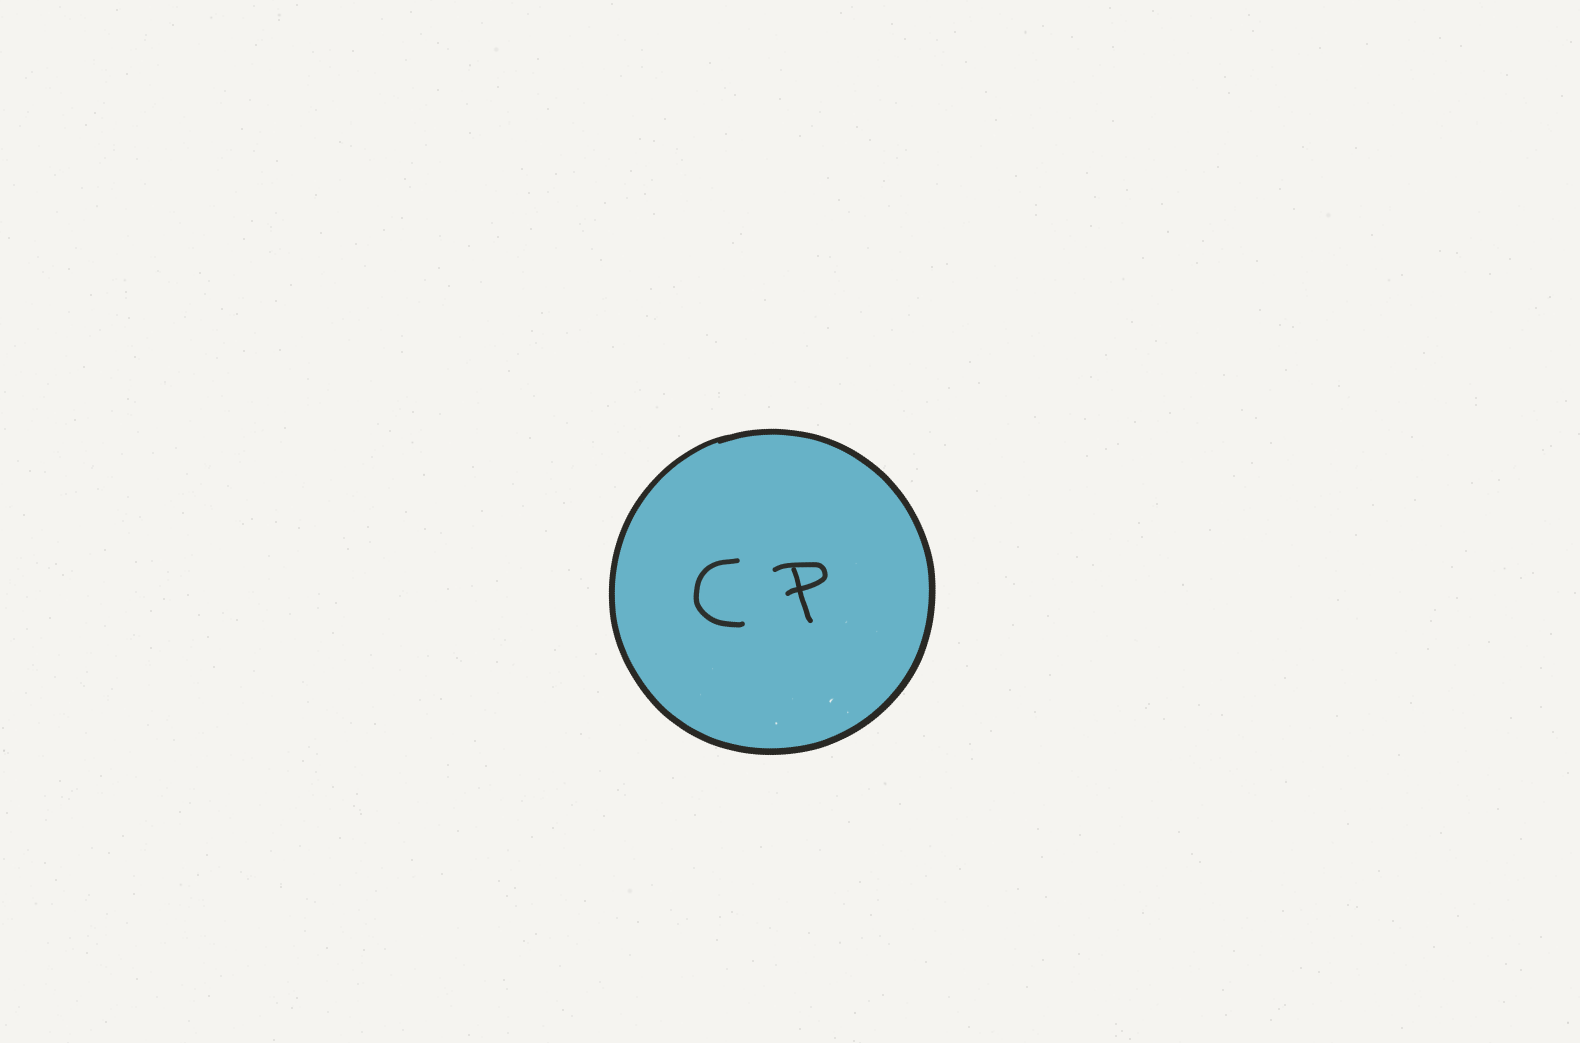
\includegraphics[height=2in]{figures/CP-cropped.png}\end{center}
    \onslide<3|handout:0>
    \begin{center}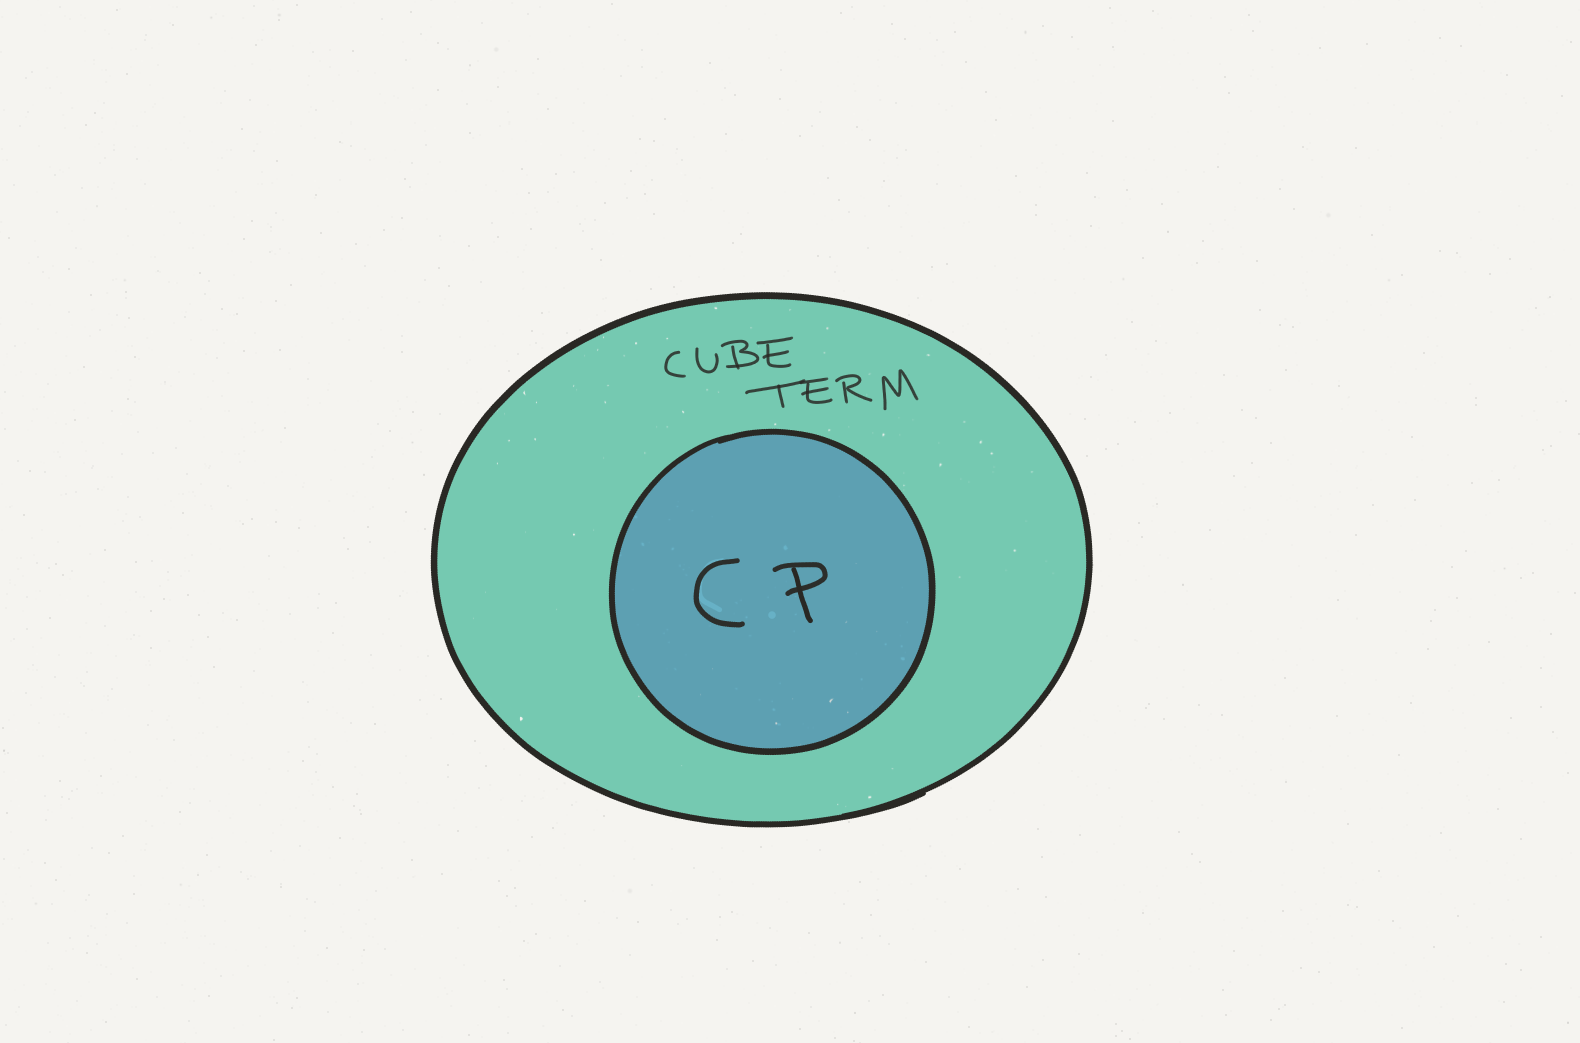
\includegraphics[height=2in]{figures/Cube-cropped.png}\end{center}
    \onslide<4|handout:0>
    \begin{center}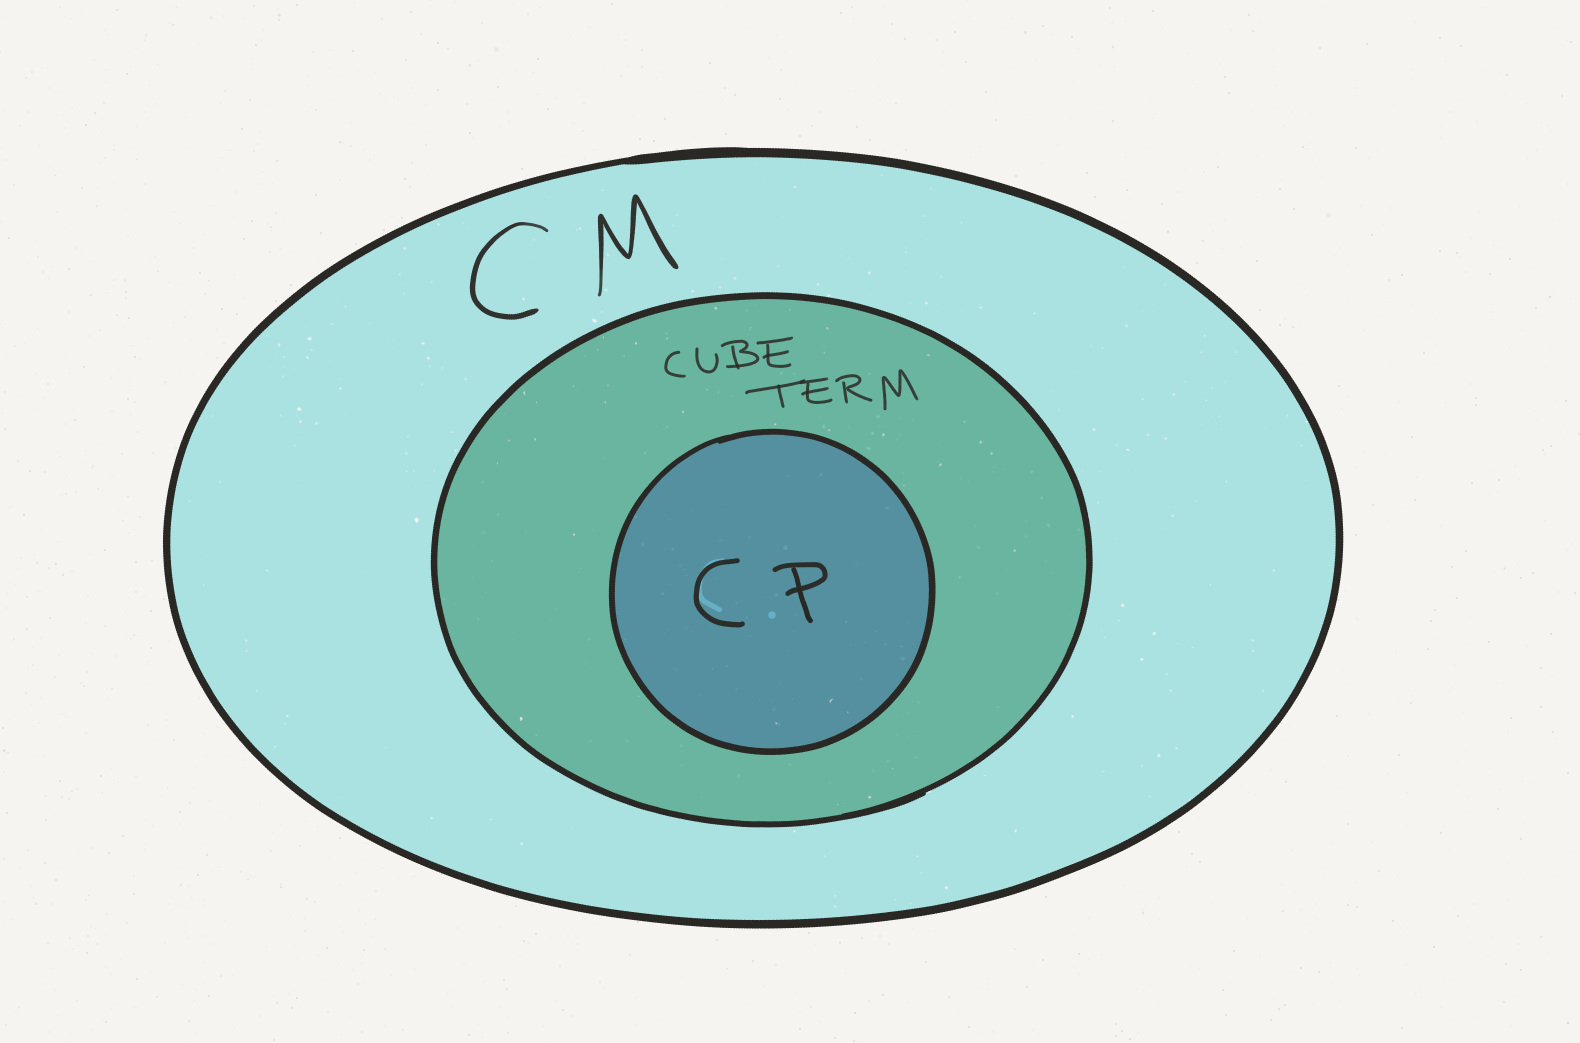
\includegraphics[height=2in]{figures/CM-cropped.png}\end{center}
    \onslide<5|handout:1>
    \begin{center}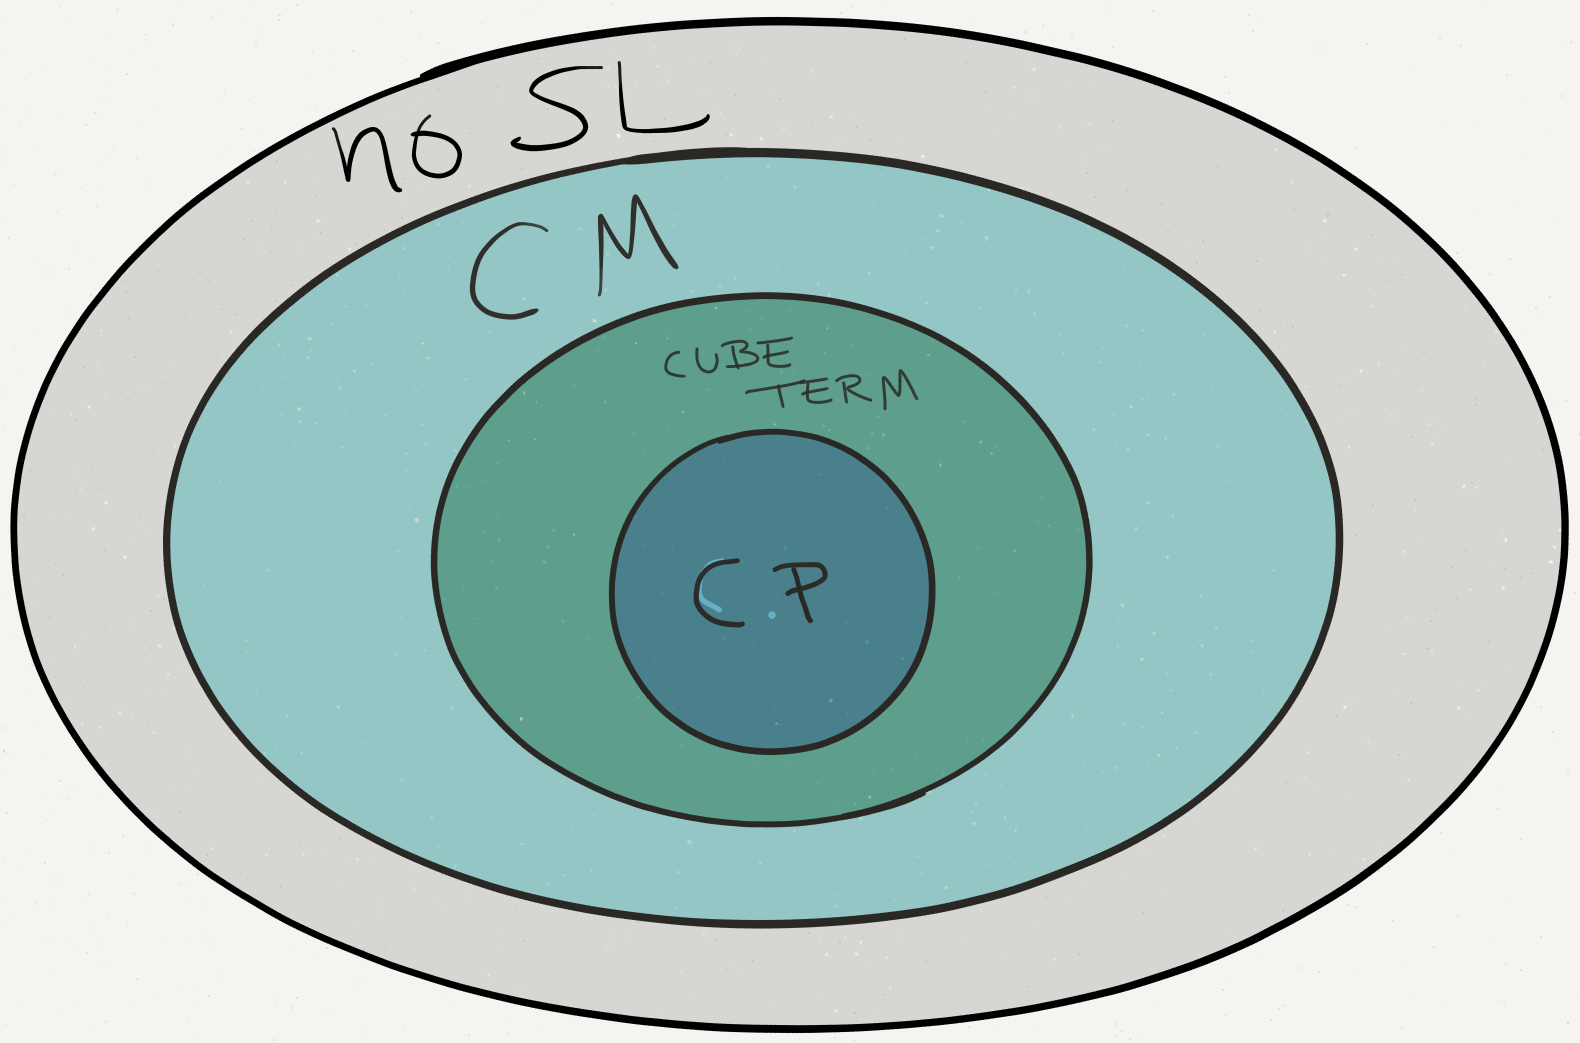
\includegraphics[height=2in]{figures/NoSL-cropped.png}\end{center}
  \end{overprint}
}




%%%%%%%%%%%%%%%%%%%%%%%%%%%%%%%%%%%%%%%%%%%%%%%%%%%%%%%%%%%
%% 10
\frame[label=cube]{
  \frametitle{First Reduction}
  \framesubtitle{by Cube-Term Blockers}

  Markovi{\'c}, M.~Mar{\'o}ti, McKenzie ($M^4$)\\
  ``Finitely related clones and algebras with cube terms'' (2012)

  \begin{block}{}
    %% \begin{definition}
    A \alert{cube-term blocker} (CTB) is a pair $(C, B)$ of subuniverses
    %% of $\bA$ 
    satisfying $\emptyset < C < B \leq A$ and for every
    $t(x_1, \dots, x_n)$ %% of $\bA$ 
    there is an index $i \in [n]$ with
    \[
    (\forall (b_1, \dots, b_n) \in B^n) (b_i \in C \longrightarrow t(b_1, \dots, b_n)\in C)
    \]
  \end{block}
    \onslide<2->
    \[
    t(b_1, \dots, b_{i-1}, c, b_{i+1}, \dots, b_n)\in C
    \]
  %% \end{definition}
  %% We call a set $D$ a (proper) \defn{ideal} of a \cib $\bA = \< A, \cdot\>$
  %%   if $D$ is a (proper) subset of $A$ satisfying $d\cdot a \in D$ for all 
  %% $d\in D$ and $a \in A$.
    \onslide<3->$M^4$ prove a finite idempotent algebra has
    a cube term iff it has no CTB.  

  \vfill
  \onslide<4->{
    \begin{lemma}
      A finite CIB $\bA$ has a CTB if and only if 
      $\bS_2 \in \sansH \sansS (\bA)$.
    \end{lemma}
    \onslide<5->{
      \begin{proof}
        $(C, B)$ a CTB implies
        $\theta = C^2 \cup (B- C)^2$ a congruence with $\bB/\theta \cong \bS_2$. 
        \\[5pt]
        Conversely, suppose $\bS_2 \in \sansH \sansS (\bA)$, and $\bB$ is 
        a subalgebra of $\bA$ with $\bB/\theta$ a meet-SL for some $\theta$. 
        Let $C/\theta$ be the bottom of $\bB/\theta$, then $(C, B)$ is a CTB.
      \end{proof}
    }
  }
}



%%%%%%%%%%%%%%%%%%%%%%%%%%%%%%%%%%%%%%%%%%%%%%%%%%%%%%%%%%%
%% 11
\frame[label=cp]{
  \frametitle{Second Reduction}

  Kearnes and Tschantz\\
  ``Automorphism groups of squares and of free algebras'' (2007)

  \begin{lemma}
    If $V$ is an idempotent variety that is not congruence permutable, then there
    are subuniverses $U$ and $W$ of $\bF := \bF_V\{x, y\}$ %% (the 2-generated free
    %% algebra)
    satisfying 
    \begin{enumerate}[1.]
    \item $x\in U \cap W$
    \item $y \in U^c \cap W^c$
    \item $(U \times F) \cup (F \times W) \leq \bF^2$
    \end{enumerate}
  \end{lemma}
  \onslide<2->{
    For CIB's, either $U$ or $W$ will be an ideal.\\[4pt]
    This implies a CTB and a semilattice.}
}


%%%%%%%%%%%%%%%%%%%%%%%%%%%%%%%%%%%%%%%%%%%%%%%%%%%%%%%%%%%
%% 12: Some well known facts
\frame[label=general2]{
  \frametitle{}

  $\bA=$ a finite CIB \hskip1cm
  $\mathbf S_2=$ the 2-elt semilattice.

  \begin{align*}
    \V(\bA) \text{ is CP } &\Longleftrightarrow \quad \bA \text{ has a Malcev term}\\
    &\Longrightarrow \quad \bA \text{ has a cube term}\\
    &\Longrightarrow \quad \V(\bA) \text{ is CM}\\
    &\Longrightarrow \quad \bS_2 \text{ is not in } \V(\bA)
    \uncover<2-|handout:2-3>{ \\   &{\mathbf \Longrightarrow} \quad \bA \text{ has a cube term} }
    \uncover<3-|handout:3>{ \\   &{\mathbf \Longrightarrow} \quad \V(\bA) \text{ is CP } }
  \end{align*}

  \begin{columns}
    \begin{column}{0.4\textwidth}
      \begin{overprint}
        \onslide<1|handout:1>
        \begin{center}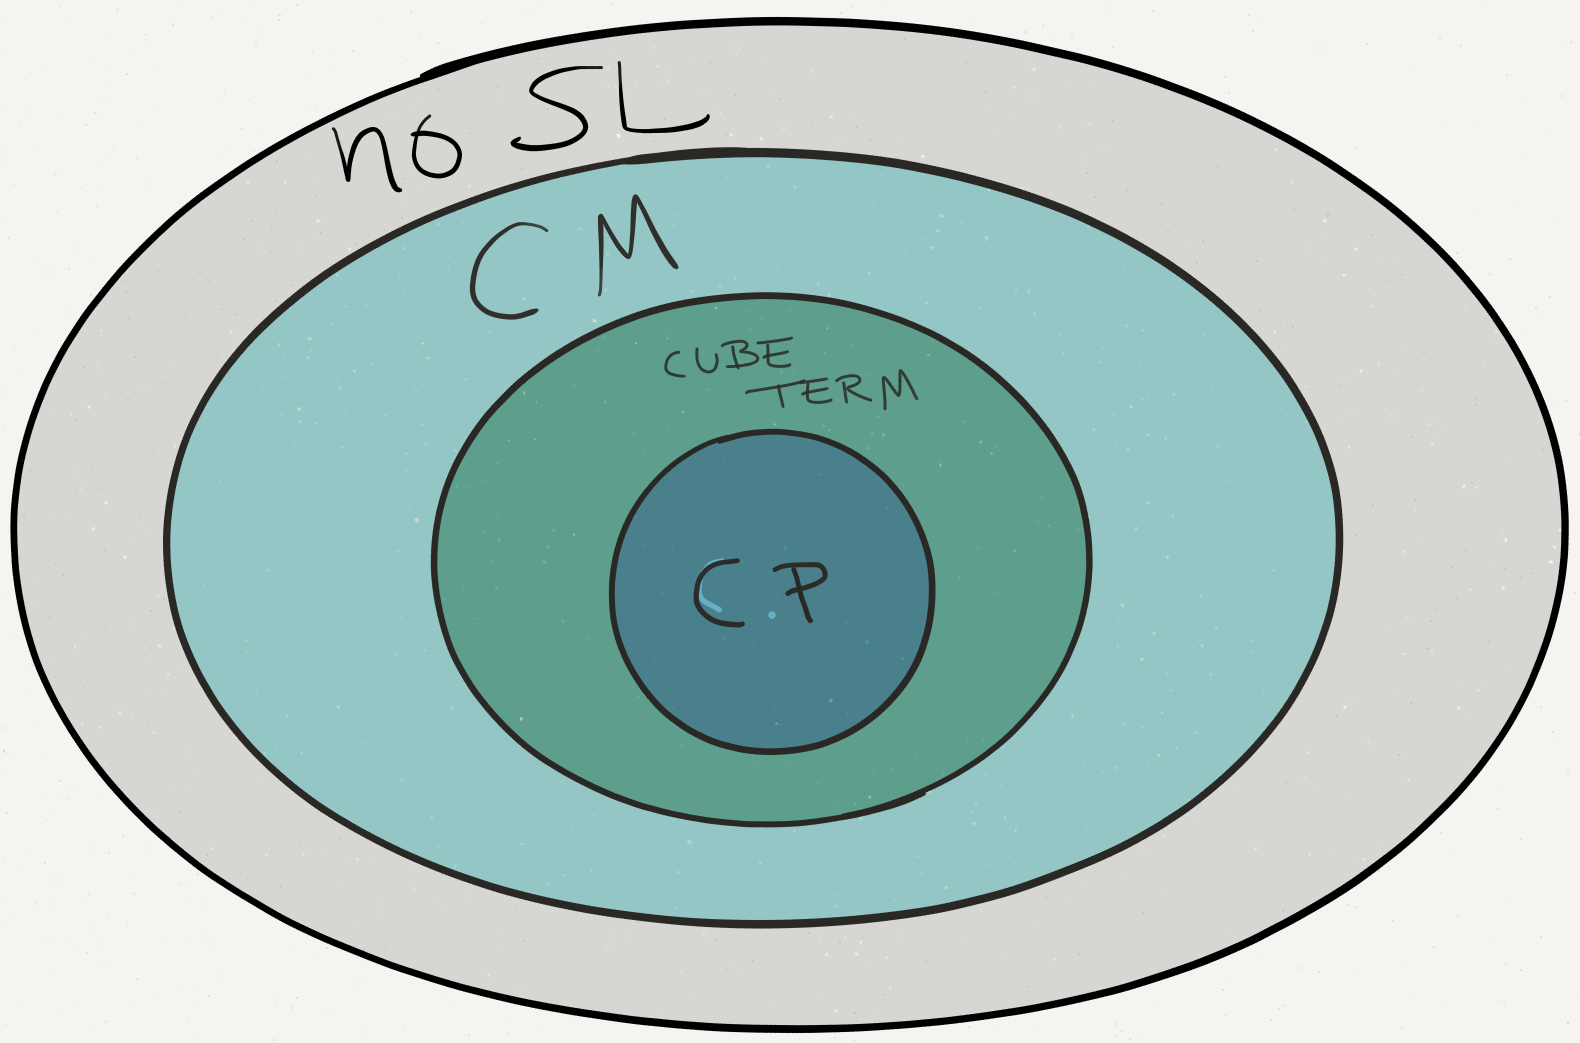
\includegraphics[height=1.25in]{figures/NoSL-cropped.png}\end{center}
        \onslide<2|handout:2>
        \begin{center}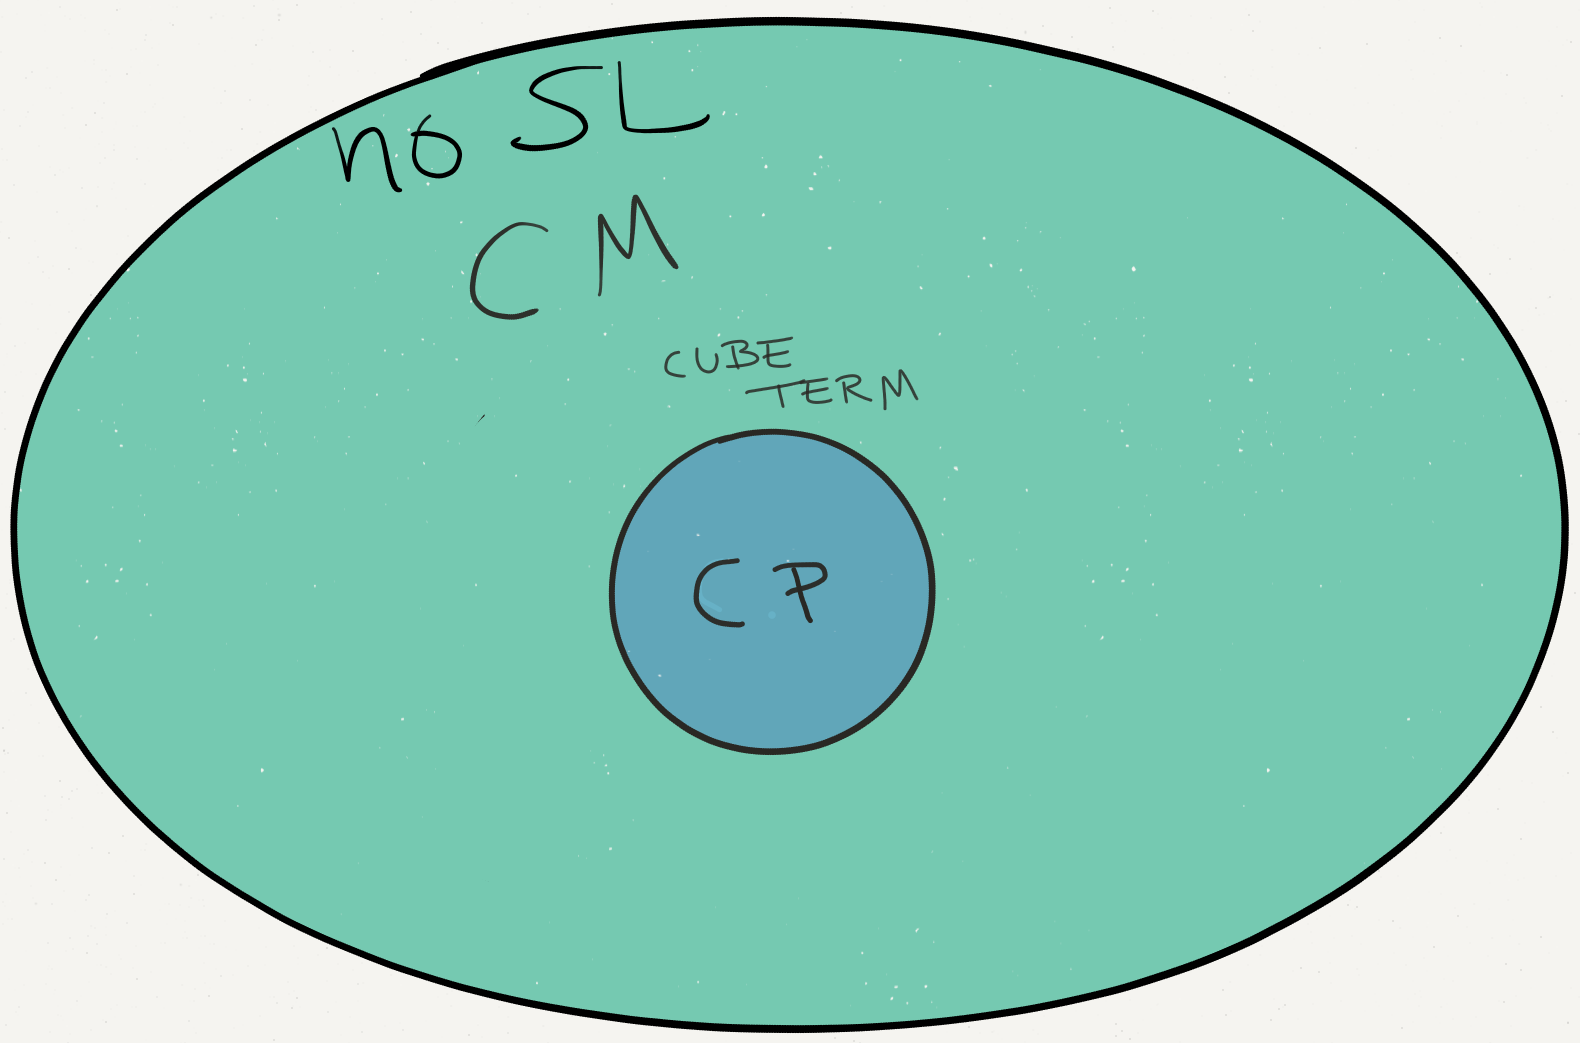
\includegraphics[height=1.25in]{figures/CubeEquiv-cropped.png}\end{center}
        \onslide<3|handout:3>
        \begin{center}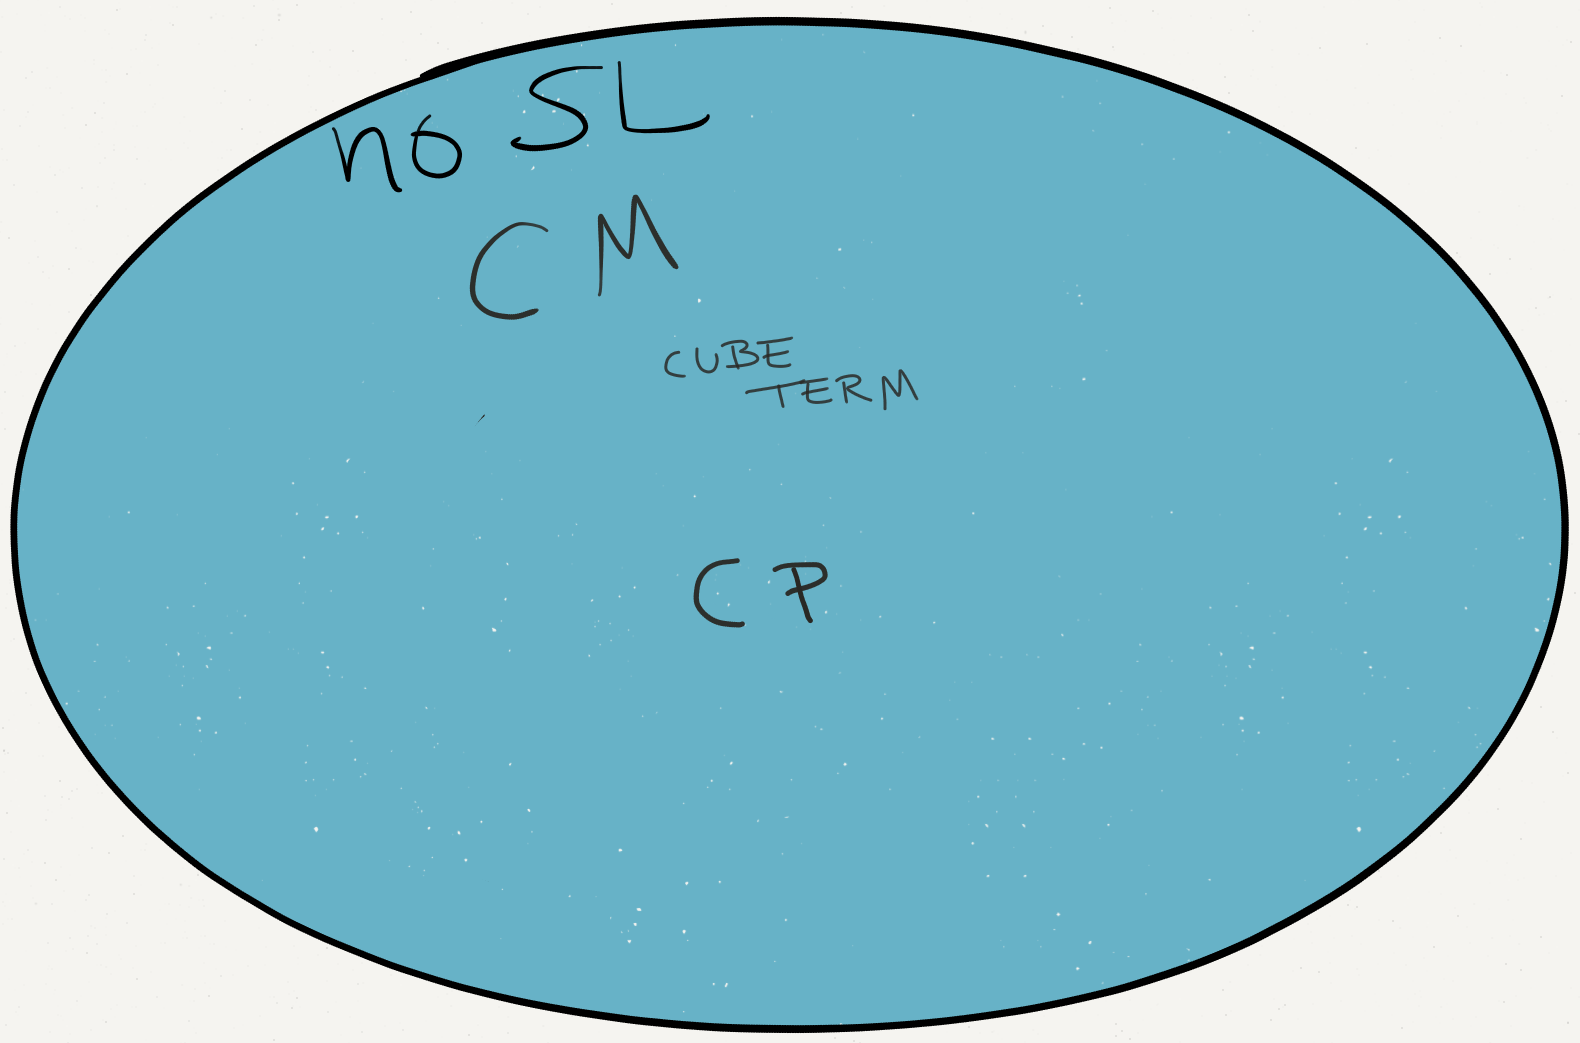
\includegraphics[height=1.25in]{figures/CPequiv-cropped.png}\end{center}
      \end{overprint}
      \vskip1cm
    \end{column}
    \begin{column}{0.6\textwidth}
        \begin{itemize}
        \item<2-|handout:2-3> 1st reduction by cube-term blockers.
        \end{itemize}
        \begin{itemize}
        \item<3-|handout:3> 2nd reduction by Kearnes-Tschantz.
        \end{itemize}
    \end{column}
  \end{columns}
}


%%%%%%%%%%%%%%%%%%%%%%%%%%%%%%%%%%%%%%%%%%%%%%%%%%%%%%%%%%%
%% 13
\frame[label=remaining]{
  \frametitle{Remaining Questions for Finite CIBs}

  \begin{block}{Conclusion}
    Let $\bA$ be a finite CIB. Then 
    \[
    \bS_2 \notin \sansH \sansS (\bA) \text{ if and
      only if } \V(\bA) \text{ is congruence permutable.}
    \]
    \onslide<2->(so $\CSP(\bA)$ tractable in this case)
  \end{block}

  \onslide<3->
  \begin{block}{Open Question}
    Let $\bA$ be a finite CIB with $\bS_2$ in $\sansH \sansS (\bA)$.  Is $\CSP(\bA)$ tractable?
  \end{block}

  \onslide<4->  Recall, 
  if $\V(\bA)$ is  $\mathrm{SD}_\wedge$, then $\CSP(\bA)$ is
  tractable.

  \onslide<5->
  \begin{block}{Revised Question}
    Let $\bA$ be a finite CIB with $\bS_2$ in $\sansH \sansS (\bA)$,
    and $\V(\bA)$ not $\mathrm{SD}_\wedge$.\\[4pt] 
    Is $\CSP(\bA)$ tractable?
  \end{block}

}

%%%%%%%%%%%%%%%%%%%%%%%%%%%%%%%%%%%%%%%%%%%%%%%%%%%%%%%%%%%
%% 14
\frame[label=examples1]{
  \frametitle{Example 1}

  \begin{columns}
    \begin{column}{0.4\textwidth}
  \begin{tabular}{c|cccc}
    $\cdot$ & 0 & 1 & 2 & 3\\
    \hline
    0 & 0 & 0 & 0 & 1\\
    1 & 0 & 1 & 3 & 2\\
    2 & 0 & 3 & 2 & 1\\
    3 & 1 & 2 & 1 & 3\\
  \end{tabular}
    \end{column}
    \begin{column}{0.6\textwidth}
      \onslide<2->
      \emph{Cliff's trick:} replace binary operation with a term from
      $\sansClo(\bA)$, say 
      \[x \ast y = (x\cdot(x\cdot y)) \cdot (y\cdot(x\cdot y))
      \]
      \\[6pt] 
      If $\<A, \ast\>$ tractable, then so is $\bA = \<A, \cdot\>$.
      \\[6pt] 
      \onslide<3->
      \begin{align*}
      \{\ast\} \subseteq \sansClo(\bA) \quad &\Longrightarrow \quad \sansRel(\sansClo(\bA)) 
      \subseteq \sansRel(\{\ast\})\\
      &\Longrightarrow \quad \CSP(\bA) \leq_P \CSP\<A, \ast\>
      \end{align*}
    \end{column}
  \end{columns}
  \onslide<4->
  \begin{columns}
    \begin{column}{0.4\textwidth}
      \begin{tabular}{c|cccc}
        $\ast$ & 0 & 1 & 2 & 3\\
        \hline
        0 & 0 & 0 & 0 & 0\\
        1 & 0 & 1 & 3 & 2\\
        2 & 0 & 3 & 2 & 1\\
        3 & 0 & 2 & 1 & 3\\
        \end{tabular}
    \end{column}
    \begin{column}{0.6\textwidth}
      $\<A, \ast\> \text{  tractable } \quad  \Longrightarrow \quad \bA 
\text{  tractable }$ 
    \end{column}
  \end{columns}
}



%%%%%%%%%%%%%%%%%%%%%%%%%%%%%%%%%%%%%%%%%%%%%%%%%%%%%%%%%%%
%% 15
\frame[label=examples2]{
  \frametitle{Example 2}

  \begin{columns}
    \begin{column}{0.4\textwidth}
  \begin{tabular}{c|cccc}
    $\cdot$ & 0 & 1 & 2 & 3\\
    \hline
    0 & 0 & 0 & 1 & 1\\
    1 & 0 & 1 & 3 & 2\\
    2 & 1 & 3 & 2 & 1\\
    3 & 1 & 2 & 1 & 3\\
  \end{tabular}
    \end{column}
    \begin{column}{0.6\textwidth}
      Let $t(x,y) = x\cdot(x\cdot(x\cdot y)) \cdot y\cdot (y\cdot(x\cdot y))$.
    \end{column}
  \end{columns}

\vskip3mm

  \onslide<2->
  \begin{columns}
    \begin{column}{0.4\textwidth}
      \begin{tabular}{c|cccc}
        $t$ & 0 & 1 & 2 & 3\\
        \hline
        0 & 0 & 0 & 0 & 1\\
        1 & 0 & 1 & 3 & 2\\
        2 & 0 & 3 & 2 & 1\\
        3 & 1 & 2 & 1 & 3\\
        \end{tabular}
    \end{column}
    \begin{column}{0.6\textwidth}
      $\<A, t\> \text{  tractable }$ 
    \end{column}
  \end{columns}
}

%%%%%%%%%%%%%%%%%%%%%%%%%%%%%%%%%%%%%%%%%%%%%%%%%%%%%%%%%%%
%% 16
\frame[label=examples3]{
  \frametitle{Example 3}

  \begin{columns}
    \begin{column}{0.4\textwidth}
  \begin{tabular}{c|cccc}
    $\cdot$ & 0 & 1 & 2 & 3\\
    \hline
    0 & 0 & 0 & 2 & 1\\
    1 & 0 & 1 & 3 & 2\\
    2 & 2 & 3 & 2 & 1\\
    3 & 1 & 2 & 1 & 3\\
  \end{tabular}
    \end{column}
    \begin{column}{0.6\textwidth}
\onslide<2->      Let $t_2(x,y) = \dots$ ?
\vskip2mm
\onslide<3->      Let $t_3(x,y,z) = \dots$ ?
    \end{column}
  \end{columns}
}
%%%%%%%%%%%%%%%%%%%%%%%%%%%%%%%%%%%%%%%%%%%%%%%%%%%%%%%%%%%
%% 17
\frame[label=others]{
  \frametitle{}
...and about 25 others.

\begin{center}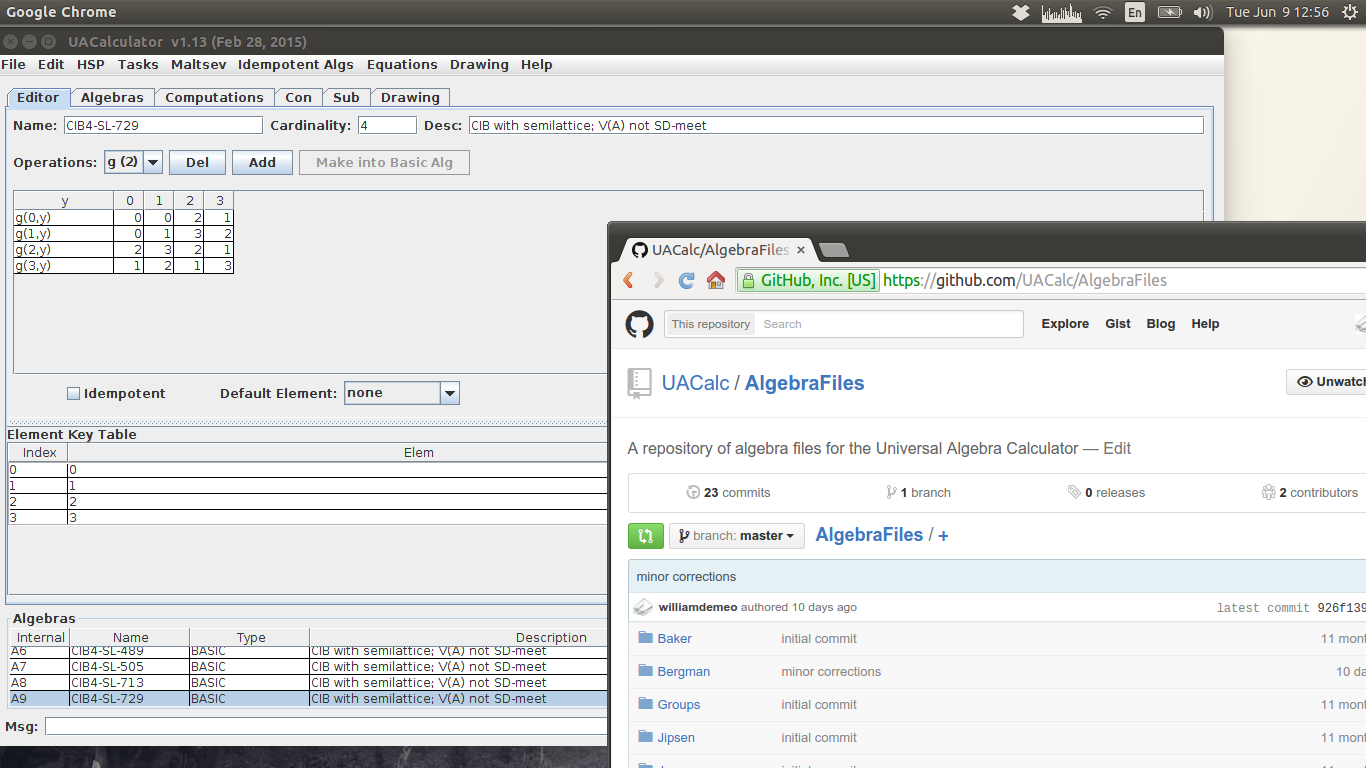
\includegraphics[height=2in]{figures/UACalcBergman.png}
%% \includegraphics[height=1.5in]{figures/BergmanDirectory.png}
\end{center}

To see them, load UACalc with files 
from the \alert{Bergman} directory at
\begin{center}
{\bf \url{https://github.com/UACalc/AlgebraFiles} }
\\[6pt]
\onslide<2->Thank you for listening!
\end{center}

}

\end{document}






Question: Does the converse of the last implication hold in general?
That is, if A is an finite idempotent algebra, then is it true that

S not in V(A)  =>  V(A) is CM?

This is certainly not true. For example, take A to be a 2-element set. However,
even if you omit type 1 it fails. Example 2.2 in the Freese-McKenzie paper on
Robust Maltsev conditions is an example. (It is actually an example due to
Matt.) You can probably find more examples by hunting through the Berman-Burris
catalog of 3-element binars:
http://www.math.uic.edu/~berman/1994-Groupoid-Catalog-Preprint.pdf 

It seems to me this is what Prop 3.9 and Cor 3.10 of Freese-Valeriote
says.  (If not, do you know a counter-example?)
No, the stuff about the tails is subtle. That's what Matt's example was designed to show.

I should know counter-examples for each of the converses that don't
hold.  Right now, I only know of one for "CM => cube term".  Namely,
the algebra Kearnes4.ua available here:

https://github.com/UACalc/AlgebraFiles/tree/master/Kearnes

has no cube term, but V(A) is CM.
This is the only example I am aware of.

What are examples of algebras with a cube term but no Malcev term.  (I
should know this! ...Jiali, feel free to jump in here!)
Every near-unanimity term is a cube term. So Lattices, for example, have cube terms but not Malcev terms. Also, the gmm terms of Dalmau are cube terms. I presume they are not always Malcev terms.

Now, back to the CIB case.  Once we prove (for CIBs) that

S not in V(A)  =>   V(A) is CP

then all the conditions above are equivalent.  That is,

For a finite CIB A, TFAE

1. V(A) is CP
2. A has a Malcev term
3. A has a cube term
4. V(A) is CM
5. S is not in V(A)
Correct. By the way, do we need A finite for this? I suspect not







